\documentclass[handout,usepdftitle=false,xcolor=dvipsnames,aspectratio=169]{beamer}
%\documentclass[beamer,usepdftitle=false,xcolor=dvipsnames,aspectratio=169]{beamer}
%\documentclass[trans,notes=show,usepdftitle=false,aspectratio=169]{beamer}


\usepackage[english]{babel}
\usepackage{iftex}
\ifPDFTeX
\usepackage[T1]{fontenc}
\usepackage[utf8]{inputenc}
\usepackage{lmodern}
\else
\usepackage{fontspec}
\defaultfontfeatures{Ligatures=TeX}
\setmainfont{Latin Modern Roman}
\setsansfont{Latin Modern Sans}
\setmonofont{Latin Modern Mono}
\usepackage{newunicodechar}
\newfontfamily\unicodeSymbolFont{Segoe UI Symbol}[
  BoldFont=Segoe UI Symbol,
  ItalicFont=Segoe UI Symbol,
  BoldItalicFont=Segoe UI Symbol
]
\newunicodechar{⟂}{{\unicodeSymbolFont ⟂}}
\fi
\usepackage{amsmath,amsfonts}
\usepackage{booktabs,multirow,xcolor,colortbl}
\usepackage{bm}%to use a more powerful version of \boldsymbol
\usepackage{fvextra}
\usepackage{csquotes}
\usepackage{textcomp}
\ifPDFTeX
\DeclareUnicodeCharacter{27C2}{\ensuremath{\perp}}
\fi

\newcommand{\AllSample}{ \mathcal Y^T }

\usepackage[citestyle=authoryear-comp,bibstyle=../Preamble/mystyle_lowercase,maxbibnames=5,minbibnames=1,maxnames=2, minnames=1,datezeros=false,date=long,isbn=false,url=false,backend=biber,useprefix=true]{biblatex}
\addglobalbib{../Preamble/Macro_database_biblatex.bib}	

\usepackage{upquote}
\usepackage{ragged2e}
\usepackage{microtype}

\usepackage{multimedia}
\usepackage{graphicx}
\usepackage[export]{adjustbox}
\usepackage{epstopdf}
\usepackage[labelfont=bf,format=hang, figurename=Fig.]{caption}
\usepackage[subrefformat=parens,labelformat=empty]{subcaption}
\usepackage{pgfpages} % for multiple-screen presentations

\usepackage{array}

\newcolumntype{L}[1]{>{\RaggedRight\let\newline\\\arraybackslash\hspace{0pt}}m{#1}}
\newcolumntype{C}[1]{>{\centering\let\newline\\\arraybackslash\hspace{0pt}}m{#1}}
\newcolumntype{R}[1]{>{\raggedleft\let\newline\\\arraybackslash\hspace{0pt}}m{#1}}
%https://tex.stackexchange.com/questions/12703/how-to-create-fixed-width-table-columns-with-text-raggedright-centered-raggedlef


%%% use serif font for math
\usefonttheme[onlymath]{serif}

%%% define blue highlighting
\newcommand{\highlight}[1]{{\color{blue}{#1}}}

%%%% define command for setting sources

\newcommand{\Source}{}

%%%
\beamertemplatenavigationsymbolsempty


%%% define themes
\usetheme{Boadilla}
\usecolortheme{rose}
\usecolortheme[named=blue]{structure}

\newcommand\textbox[1]{%
  \parbox{.333\textwidth}{#1}%
}

\setbeamertemplate{sections/subsections in toc}[sections numbered]


%%%% set coloring in  foot and head
\setbeamercolor{alerted text}{fg=red!80!black}
\setbeamertemplate{enumerate items}[default] % numbers enumerate items without encircling them
\setbeamertemplate{itemize items}[ball] % numbers enumerate items without encircling them
\setbeamercolor{section in head/foot}{fg=black, bg=white}
\setbeamercolor{subsection in head/foot}{fg=black, bg=white}
\setbeamercolor{title}{fg=black}
\setbeamercolor{subtitle}{fg=blue}

\setbeamertemplate{caption}[numbered]

%%% set overlays as default
\beamerdefaultoverlayspecification{<+->}

%%%% settings for output mode

\mode<beamer>
{
%\setbeameroption{show notes on second screen=right}
}

\mode<trans>
{\renewcommand{\highlight}[1]{{\textbf{#1}}}}


\mode<handout>
{
\renewcommand{\highlight}[1]{{\textbf{#1}}}
%\pgfpagesuselayout{4 on 1}[a4paper,border shrink = 5mm,landscape]
%\setbeamercolor{background canvas}{bg=black!5}
}


%%% define Exercise counter
\newcounter{Exercise}
\resetcounteronoverlays{Exercise}
\setcounter{Exercise}{0}
\newcommand{\Exercise}{\refstepcounter{Exercise}\emph{\structure{Übung \theExercise}: }}

%%%% define environments for theorems etc and make them numbered
\setbeamertemplate{theorems}[numbered]

\newtheorem{assum}{Assumption}
\setbeamertemplate{assum}[numbered]

\newtheorem{defin}{Definition}
\setbeamertemplate{defin}[numbered]

\newtheorem{propos}{Proposition}
\setbeamertemplate{propos}[numbered]


%%%% Make Parts show up in TOC
\makeatletter
\AtBeginPart{%
  \addtocontents{toc}{\protect\beamer@partintoc{\the\c@part}{\beamer@partnameshort}{\the\c@page}}%
}
%% number, shortname, page.
\providecommand\beamer@partintoc[3]{%
  \ifnum\c@tocdepth=-1\relax
    % requesting onlyparts.
    \makebox[6em]{#1.} #2
    \par
  \fi
}
\define@key{beamertoc}{onlyparts}[]{%
  \c@tocdepth=-1\relax
}
\makeatother%

%%%% fix bug in beamer package with note itemize
%%% http://tex.stackexchange.com/questions/1480/changing-the-textwidth-of-the-notes-in-beamer-repost-from-so
\makeatletter
\defbeamertemplate{note page}{infolines}
{%
  \vskip.75em
  \nointerlineskip
  \begin{minipage}{\textwidth} % this is an addition
  \footnotesize \insertnote
  \end{minipage}               % this is an addition
}
\makeatother

\setbeamertemplate{note page}[infolines]


\newcommand{\backupbegin}{
   \newcounter{framenumberappendix}
   \setcounter{framenumberappendix}{\value{framenumber}}
}
\newcommand{\backupend}{
   \addtocounter{framenumberappendix}{-\value{framenumber}}
   \addtocounter{framenumber}{\value{framenumberappendix}}
}

\hypersetup{bookmarksnumbered=true,naturalnames=true,pdfhighlight=/N,citebordercolor={1 1
1},linkbordercolor={1 1 1},colorlinks=true,anchorcolor=black,linkcolor=blue,citecolor=green,urlcolor=green,
pdfpagemode=UseOutlines,breaklinks=true,
pdfkeywords=Dynare, pdfsubject=Dynare,pdfstartpage=1} %pdfpagemode=fullpage

\usepackage[copyright]{ccicons}

\usepackage{tikz,pgfplots}
\pgfplotsset{compat=1.18}
\usetikzlibrary{arrows,calc,decorations.pathreplacing,decorations.shapes}
\pgfdeclarelayer{background}
\pgfdeclarelayer{foreground}
\pgfsetlayers{background,main,foreground}

\usepackage{relsize}
\newcommand\LM{\ensuremath{\mathit{LM}}}
\newcommand\IS{\ensuremath{\mathit{IS}}}
\DeclareMathOperator{\std}{std}


\setbeamertemplate{footline}{
\begin{beamercolorbox}{subsection in head/foot}
\insertsectionnavigationhorizontal{.95\textwidth}{\hskip0pt
\hfill}{\hfill \insertframenumber /\inserttotalframenumber}
\end{beamercolorbox}
}

\newenvironment{witemize}{\itemize\addtolength{\itemsep}{8pt}}{\enditemize}
\newenvironment{wenumerate}{\enumerate\addtolength{\itemsep}{8pt}}{\endenumerate}

\usepackage[]{minted}
\usepackage{tcolorbox}
\usepackage{etoolbox}
\BeforeBeginEnvironment{minted}{\begin{tcolorbox}[boxsep=0mm]}%
\AfterEndEnvironment{minted}{\end{tcolorbox}}%

\AtBeginEnvironment{minted}{%
  \renewcommand{\fcolorbox}[4][]{#4}}  

\newcommand{\AllSample}{ \mathcal Y^T }


\AtBeginSection[]{
  \begin{frame}[plain]
  \frametitle{Overview}
  \tableofcontents[currentsection,hideallsubsections]
  \end{frame}
}

\title[]{\textbf{Advanced Dynare\\}
\medskip{Chapter VI}\\
\emph{Full information estimation of DSGE models}
}

\author{Johannes Pfeifer}
\input{../date_place.txt}


\begin{document}

\maketitle

% LTeX: language=en-US

\begin{frame}{Review}
\begin{witemize}
\item Log-Linearized DSGE model solution takes state-state space form\vspace{0.2cm}
\item Typically, not all state variables are observed\vspace{0.2cm}
\item Solution: use Kalman Filter to deal with unobserved states and construct likelihood\vspace{0.2cm}
\item Result: likelihood $\mathcal{L}(y^T|\theta)$, where $\theta$ is the vector of deep parameters and $y^T$ is the complete history of observables \vspace{0.2cm}
\item Estimating meant finding the parameters $\theta$ that maximized $\mathcal{L}(y^T|\theta)$
\end{witemize}

\end{frame}


\section[The Problem]{The problem addressed by Bayesian estimation}
%\renewcommand{\Source}{Maddison Data Set}

\begin{frame}{The likelihood}
\begin{columns}<.->[T] % align columns
\begin{column}<.->{0.4\textwidth}
\begin{witemize}
\item The likelihood is a high-dimensional object\medskip
\item Even for simple models, it can be ill-behaved, showing hardly any curvature and exhibiting many local maxima
\end{witemize}
\end{column}%
\hfill% 
\begin{column}<1->{0.6\textwidth}
\begin{figure}
  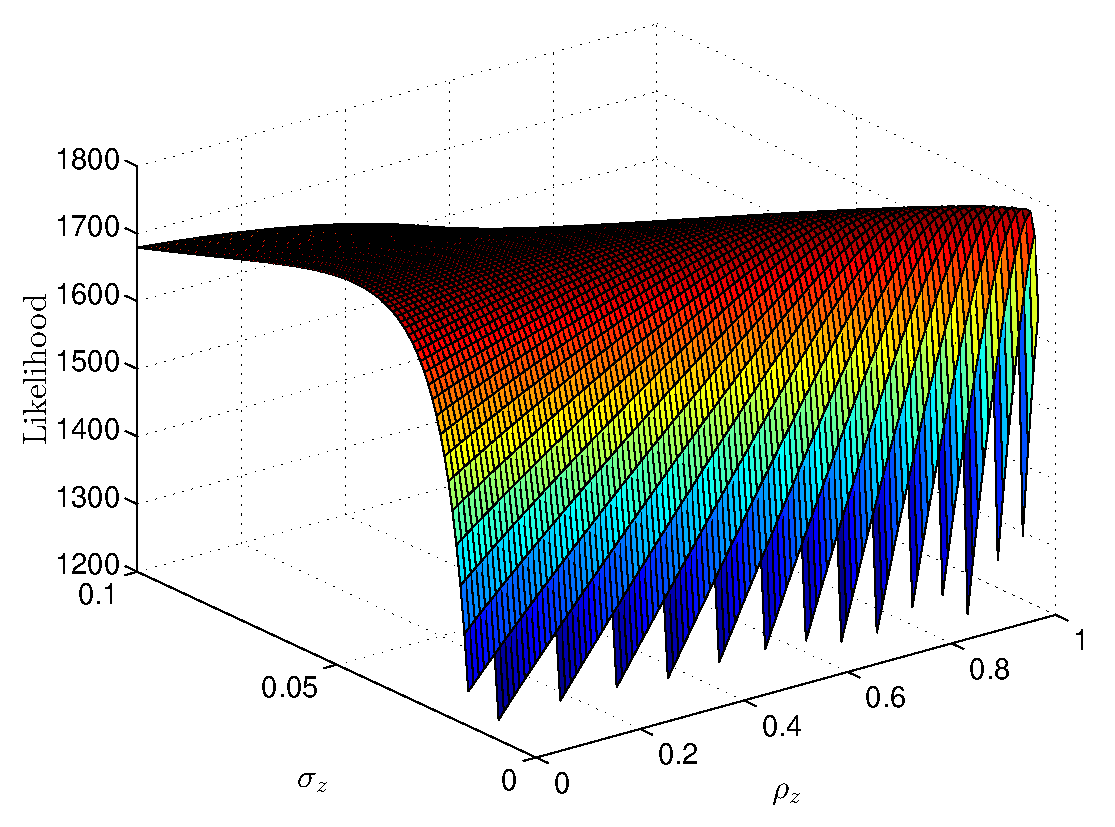
\includegraphics[scale=.45]{Figures/likelihood_surf}
\end{figure}

\end{column}%
\end{columns}

\end{frame}

\begin{frame}{The likelihood}
\begin{columns}<.->[T] % align columns
\begin{column}<.->{0.4\textwidth}
\begin{witemize}
\item For more complicated models, you can think of it as an egg-crate\medskip
\item ``Dilemma of absurd parameter estimates'' \parencite{AnSchorfheide2007}: ML estimates often at odds with information from outside the model
\end{witemize}
\end{column}%
\hfill%
\begin{column}<1->{0.6\textwidth}
\begin{figure}
   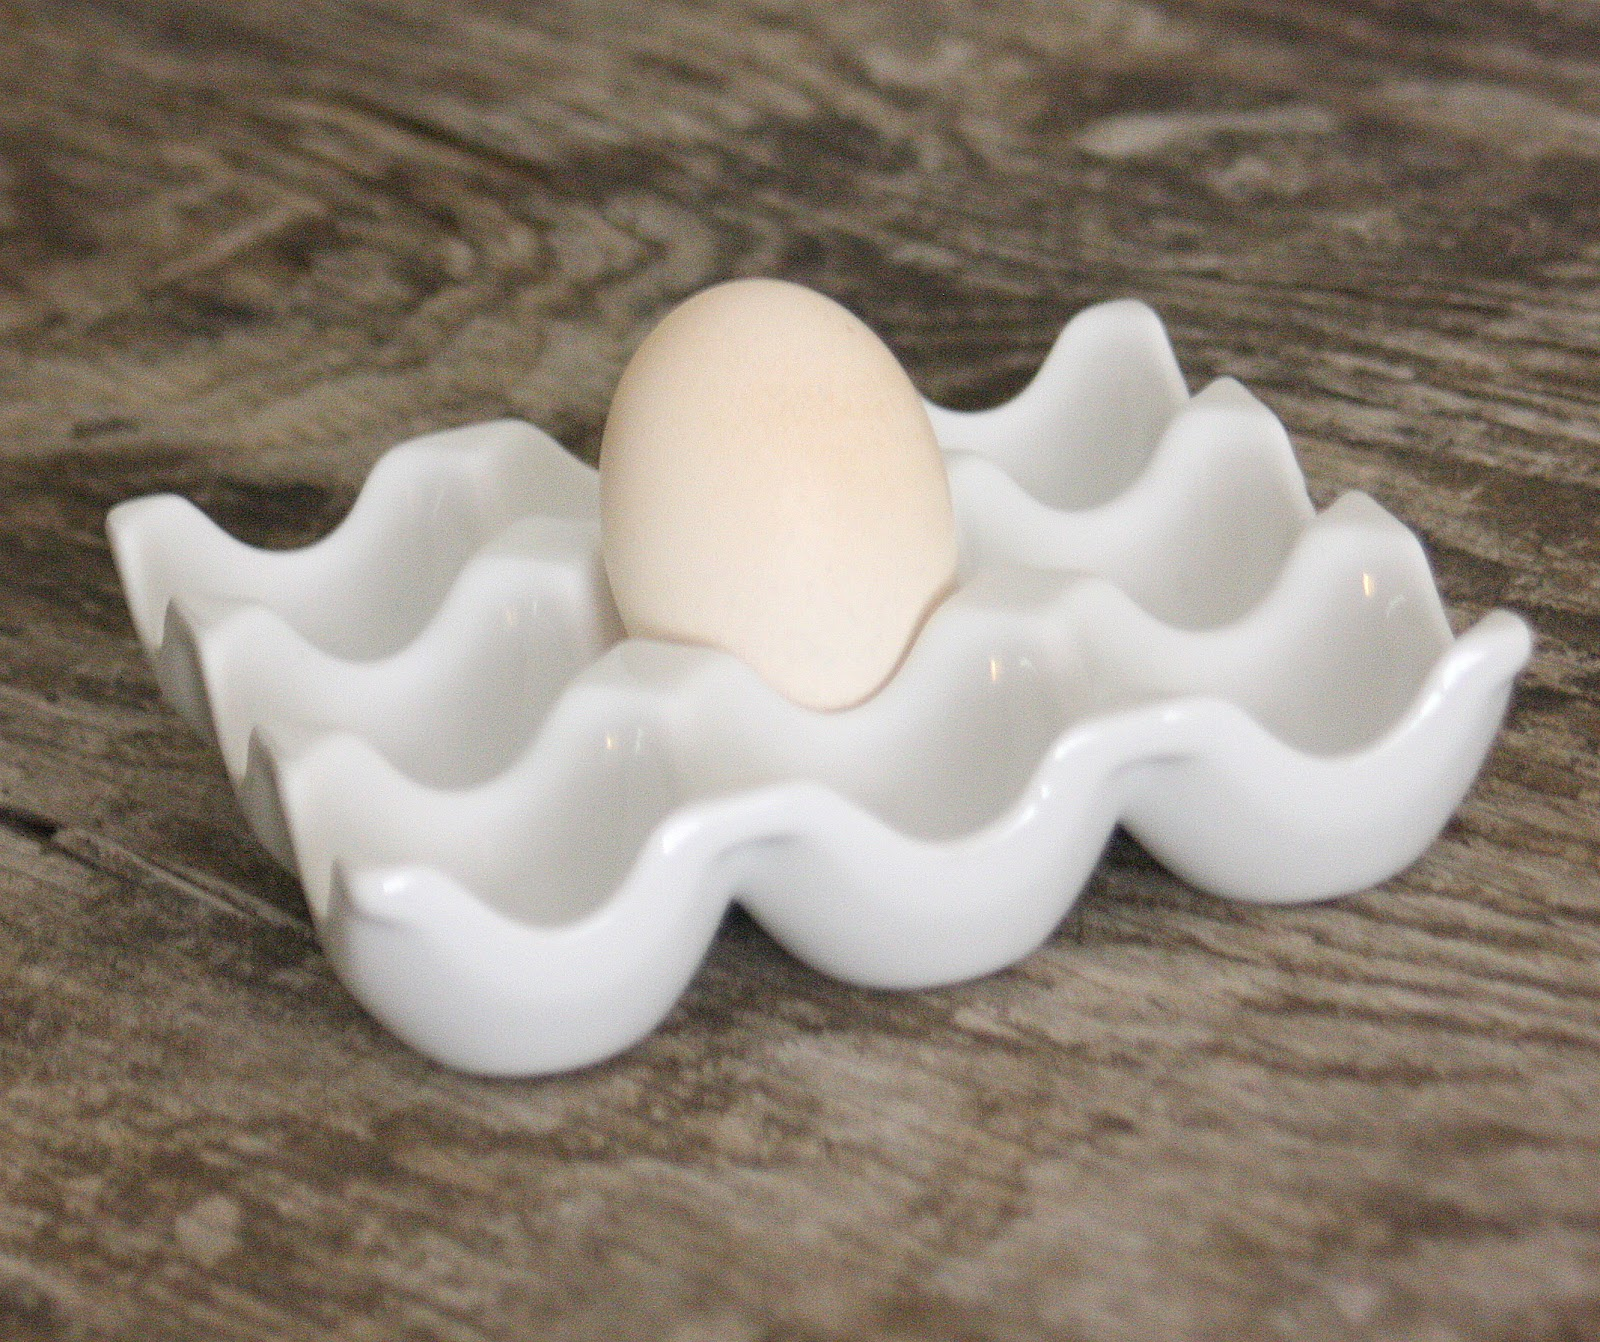
\includegraphics[scale=.1]{Figures/egg_crate}
\end{figure}

\end{column}%
\end{columns}


\end{frame}


\renewcommand{\Source}{\textcite{Koop2003}, Ch. 1}
\begin{frame}{Bayesian vs.\ frequentist philosophy}
\begin{witemize}
    \item In principle, there is a fundamental philosophical difference between Bayesian and frequentist econometrics
%    \item For example, frequentists, the data are treated as random variables and the parameters as fixed, for Bayesians, the data are fixed and the parameters are random variables
%    \item Moreover, Bayesians incorporate ``subjective'' prior information, while frequentists claim ``objectivity'' (although model choice, data selection etc. also involve subjective choices)
    \item Most macroeconomists are not Bayesian believers but pragmatists - up to the point that Bayesian and frequentist techniques are used in the same papers
    \item Adopting Bayesian techniques makes our lives easier
    \item Historically, Bayesian were the minority because computing power was not sufficient to apply their methods
    \item There are very good reasons to be Bayesian \parencite[see e.g.][]{BergerWolpert1988,Sims2007}
\end{witemize}
\end{frame}

\renewcommand{\Source}{\textcite{ZyphurOswald2013}}
\begin{frame}{Bayesian vs.\ frequentist philosophy: concept of probability}
\begin{witemize}
    \item Bayesian probability is usually associated with \highlight{degrees of belief or degrees of knowledge}
    \item Frequentist probability is usually based on \highlight{features of hypothetically observable systems}\\
    $\rightarrow$ relative frequency of an event ``in the long run''
    \item Example: ``There is a .50 probability that a fair coin will land heads.''\\
    \begin{itemize}
      \item Bayesian: belief evenly divided between the coin landing heads or tails
      \item Frequentist: result if coin were flipped a hypothetical infinite number of times
    \end{itemize}
    \item Frequentist analysis limited to inference about relative frequency of events in the long run
    \item But: long run unobservable and not in researchers' actual interest
    \item Bayesians can apply probability to anything that can be the subject of belief or knowledge (hypotheses, statistical parameters, entire statistical models)
\end{witemize}
\end{frame}

\begin{frame}{Bayesian vs.\ frequentist philosophy: conditioning sets}
\begin{witemize}
    \item Frequentists estimate sampling distribution for estimated effect/parameter
    \begin{itemize}
      \item distribution simulates observed effect if repeated infinite number of times, with only sampling error affecting results
      \item data carry uncertainty via sampling distribution, while parameter has fixed ``true'' population value\\
      $\rightarrow$ \highlight{conditioning on parameter} $P(Y|\theta)$
      \item Null Hypothesis Significance Testing (NHST) involves testing a hypothesis we do not believe in
      \item $p$-value gives probability of effect, assuming Null is true\\
      $\rightarrow$ relies on hypothetically repeating experiment that never occurred
    \end{itemize}
    \item Bayesians make direct probabilistic statements about effect/parameter, based on observed data
    \begin{itemize}
      \item Parameter is treated as random/uncertain while data is taken as fixed\\
      $\rightarrow$ \highlight{conditioning on data} $P(\theta|Y)$
    \end{itemize}
\end{witemize}
\end{frame}

\renewcommand{\Source}{\textcite{Koop2003}, Ch. 1}
\begin{frame}{The posterior density}
\begin{witemize}
    \item Central object: \highlight{posterior probability/posterior density}
    \begin{equation}
      P(\theta|Y)
    \end{equation}
    of a parameter $\theta$, conditional on having seen the data $Y$
    \item Posterior is fully-fledged density function!
    \item Allows statements like: the regression indicates that with 90\% probability the fiscal multiplier is between 0.3 and 1.5
    \item NHST does not allow such statements!
    \item Rejecting the Null does not tell us anything about likely effect\\
    $\rightarrow$ only know the data is unlikely to come from a world where the Null is true\\
    $\rightarrow$ estimated value is then preferred
    \item Problem: how to obtain this posterior?
\end{witemize}
\end{frame}

\begin{frame}{The central element: Bayes' Rule}
\begin{witemize}
    \item Consider the basic laws of probability for two events $A$ and $B$:
    \begin{align}
        p\left( {A,B} \right) &= p\left( {A|B} \right)p\left( B \right) \\
        p\left( {A,B} \right) &= p\left( {B|A} \right)p\left( A \right)
    \end{align}
    where $p\left( {A,B} \right)$ is the joint probability, $p\left( {A|B} \right)$ is the conditional probability, and $p\left( B \right)$ the marginal probability
    \item Equating them results in \highlight{Bayes' Rule}
    \begin{equation}
    p\left( {B|A} \right) = \frac{{p\left( {A|B} \right)p\left( B \right)}}{{p\left( A \right)}}
    \end{equation}
\end{witemize}
\end{frame}


\begin{frame}{Bayes' Rule applied}
\begin{witemize}
    \item Now apply this to a case where we want to use some data $y^T$ to infer a parameter vector $\theta$
        \begin{equation}
            p\left( {\theta |{y^T}} \right) = \frac{\mathcal{L}\left( {{y^T}|\theta } \right)p\left( \theta  \right)}{p\left( y^T \right)} \propto \mathcal{L}\left( {{y^T}|\theta } \right)p\left( \theta  \right) \label{eq:Bayes}
        \end{equation}
    \item $p\left( {\theta |{y^T}} \right)$ is called the \highlight{posterior distribution}; it incorporates all we know about the parameters and incorporates data and non-data information
    \item $p\left( \theta \right)$ is the \highlight{prior distribution}; it is independent of the data and incorporates all non-data information on the parameters
    \item $p\left( y^T \right)$ is the \highlight{data density}; as it is independent of the parameters, it can be treated as a proportionality constant (except when doing model comparison)
    \item Equation \eqref{eq:Bayes} says that the \highlight{posterior is proportional to likelihood times prior}
\end{witemize}
\end{frame}


\begin{frame}{The problem with Bayesian estimation}
\begin{itemize}
    \item Historically, Bayesians were the minority due to insufficient computing power. Why?
    \item
        \begin{equation}
            p\left( {\theta |{y^T}} \right) = \frac{\mathcal{L}\left( {{y^T}|\theta } \right)p\left( \theta  \right)}{p\left( y^T \right)} \propto \mathcal{L}\left( {{y^T}|\theta } \right)p\left( \theta  \right) \tag{\ref{eq:Bayes}}
        \end{equation}
        describes a \highlight{full distribution} that often is not analytically tractable
    \item Characterizing the posterior distribution by its mean and variance. We need to compute:
    \begin{equation}
    \mathbb{E}\left( {\theta |{y^T}} \right) = \int {\theta p\left( {\theta |{y^T}} \right)d\theta }
    \end{equation}
    and
    \begin{align}
      \operatorname{var} \left( {\theta |{y^T}} \right) &= \mathbb{E}\left( {{\theta ^2}|{y^T}} \right) - {\left[ {\mathbb{E}\left( {\theta |{y^T}} \right)} \right]^2} \notag \\
       &= \int {{\theta ^2}p\left( {\theta |{y^T}} \right)d\theta }  - {\left[ {\mathbb{E}\left( {\theta |{y^T}} \right)} \right]^2}
    \end{align}
    \item We need to evaluate integrals that usually cannot be worked out analytically!
    \end{itemize}
\end{frame}

\section[Posterior]{Characterizing the posterior}
\begin{frame}{Getting the mean}
\begin{witemize}
    \item Ingenious idea: we are typically interested in integrals of the form
    \begin{equation}
    \mathbb{E}\left( {g\left( \theta  \right)|{y^T}} \right) = \int {g\left( \theta  \right)p\left( {\theta |{y^T}} \right)d\theta }
    \end{equation}
    \item If we had \highlight{iid draws from the posterior}, we could simply use a law of large numbers:
    \begin{equation}
    \mathbb{E}\left( {g\left( \theta  \right)|{y^T}} \right) = \int {g\left( \theta  \right)p\left( {\theta |{y^T}} \right)d\theta }  \approx \frac{1}{S}\sum\limits_{s = 1}^S {g\left( {{\theta _s}} \right)} =\hat g_S
    \end{equation}
    \item Replace integral by sum over $S$ draws from the posterior distribution $p(\theta|y^T)$
    \item This is called \highlight{Monte Carlo Integration}
    \end{witemize}
\end{frame}

\begin{frame}{Numerical standard error}
\begin{itemize}
    \item How good is this estimate?
    \item Central limit theorem ensures that
        \begin{equation}
        \sqrt S \left( {{{\hat g}_S} - \mathbb{E}\left( {g\left( \theta  \right)|{y^T}} \right)} \right) \to N\left( {0,\sigma _g^2} \right)
        \end{equation}
    \item Hence,
    \begin{equation}
    \mathbb{E}\left( {g\left( \theta  \right)|{y^T}} \right) \sim N\left( {{{\hat g}_S},\frac{{\sigma _g^2}}{S}} \right)
    \end{equation}
    \item The standard deviation
        \begin{equation}
        \sigma _g^2=\operatorname{var}(g(\theta)|y^T)
        \end{equation}
        can be estimated by the variance in our Monte Carlo sample
    \item The \highlight{Numerical Standard Error (NSE)}
    \begin{equation}
    \frac{{\sigma _g}}{\sqrt S}
    \end{equation}
    is a measure of approximation error.
\end{itemize}
\end{frame}

\renewcommand{\Source}{\textcite{Koop2003}, p. 44}
\begin{frame}{Some more jargon}
\begin{itemize}
    \item Even if you are not a Bayesian believer, you should be familiar with the different terminology
    \item Denote with $\omega=g(\theta)$ some vector of functions of the parameters $\theta$, defined over some region $\Omega$
\end{itemize}
      \begin{Definition}[Credible Set]
      The set $C\subseteq \Omega$ is a $100(1-\alpha)\%$ \highlight{credible set} with respect to $p(\omega|y)$ if
      \vspace{-.3cm}
      \begin{equation}
      p(\omega \in C|y)=\int_C p(\omega|y)d\omega=1-\alpha
      \end{equation}
    \end{Definition}
\begin{itemize}
    \item We are typically interested in the smallest one, the ``Bayesian equivalent to a confidence interval''
\end{itemize}
      \begin{Definition}[Highest Posterior Density Interval]
      A $100(1-\alpha)\%$ \highlight{highest posterior density interval} for $\omega$ is a $100(1-\alpha)\%$ \highlight{credible interval} that has a smaller support than any other $100(1-\alpha)\%$ credible interval for $\omega$
    \end{Definition}
\end{frame}

%\renewcommand{\Source}{\textcite{Sims2007}/\textcite{BergerWolpert1988}}
%\begin{frame}{Credible Set vs. Confidence Intervals}
%\begin{itemize}
%    \item Bayesian credible sets are \highlight{post-experimental}: conditional upon observing the data, a $(1-\alpha)\%$ credible set contains the true parameter, which is a random variable, with $(1-\alpha)\%$ probability
%    \item Frequentist confidence intervals are based on the long-run performance if an experiment is repeatedly performed
%    \item They are thus inherently \highlight{pre-experimental} and treat the parameter as non-random
%    \item CIs are constructed so that the true parameter will be contained in $(1-\alpha)\%$ of the CI constructed from the data
%    \item Moreover, a $(1-\alpha)\%$ CI contains the true parameter value with probability $(1-\alpha)\%$ only before one has seen the data
%    \item After the data has been seen, the probability is zero or one
%    \item CIs do not help in putting constraints on a parameter after data is observed
%    \item One can only say: the true parameter is either in the CI or not
%    \item Thus, both answer fundamentally different questions
%\end{itemize}
%\end{frame}
%
%\begin{frame}{Credible Set vs. Confidence Intervals: Example}
%\begin{itemize}
%    \item We want to infer a parameter $\theta$ and observe two independent random variables $X_1$ and $X_2$ with
%      \[
%      P(X_i=\theta-1)=P(X_i=\theta+1)=0.5 \: , i \in 1,2
%      \]
%      \item The smallest 75\% CI is
%      \[
% C\left( {{X_1},{X_2}} \right) = \left\{ {\begin{array}{*{20}{c}}
%  {\frac{1}{2}\left( {{X_1} + {X_2}} \right)\: \text{if} \: {X_1} \ne {X_2}} \\
%  {X_1} - 1 \: \text{if} \: {X_1} = {X_2}
%\end{array}} \right.
%\]
%    \item When repeatedly sampling, the true $\theta$ will be in this interval in $75\%$ of the cases, because
%    \begin{itemize}
%        \item if ${x_1} \ne {x_2}$ (half of the cases), we know for sure that $\theta=0.5(x_1+x_2)$\\
%        $\Rightarrow$ correct in $100\%$ of these cases
%        \item if ${x_1} = {x_2}$ (half of the cases), either $\theta=x_1+1$ or $\theta=x_1-1$\\
%        $\Rightarrow$ correct in $50\%$ of these cases
%    \end{itemize}
%\item Bayesians, upon observing the data, are $100\%$ sure about $\theta$ or $50\%$
%\item Does it make sense to report pre-experimental measure when it is known to be misleading after seeing the data?
%\end{itemize}
%\end{frame}

\renewcommand{\Source}{}
\begin{frame}{Problems everywhere: posterior sampling}
\begin{witemize}
    \item Monte Carlo Integration sounds nice and easy, but there's a problem: how to get draws from an intractable distribution?
    \item This is the big topic of \highlight{posterior sampling algorithms}
    \item The most important ones are
    \begin{itemize}
      \item Importance Sampling
      \item Gibbs-Sampling \parencite{GemanGeman1984}
      \item Metropolis-Hastings algorithm \parencite{Metropolis1953,Hastings1970}
    \end{itemize}
    \item We will only consider the last one
    \item Gibbs-Sampler is a special case of the Metropolis-Hasting algorithm \parencite[see][]{Gelman1992}
    \item Gibbs sampling and the Metropolis-Hastings algorithm give rise to \highlight{correlated random draws from the posterior} and belong to the class of \highlight{Monte Carlo Markov Chain} algorithms
\end{witemize}
\end{frame}

\section[Prior]{Prior distributions}

\begin{frame}{Where do priors come from?}
\begin{figure}
  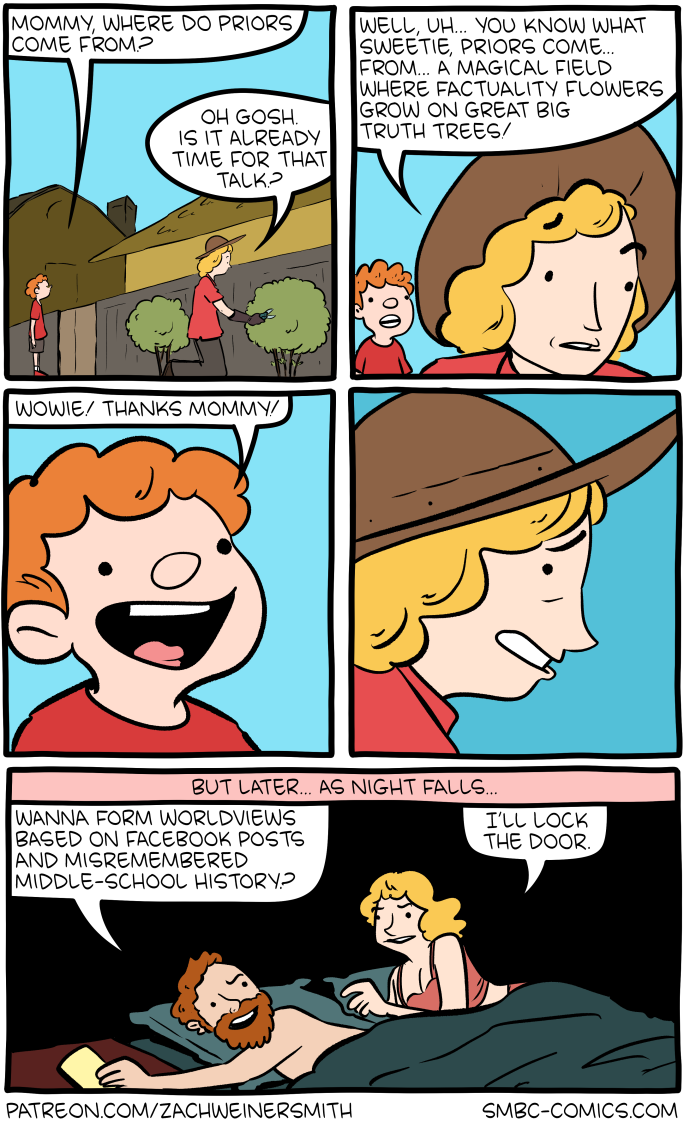
\includegraphics[trim=0 370 0 0,clip,width=6 cm]{Figures/SMBC_1759360612-20251002_priors.png}
  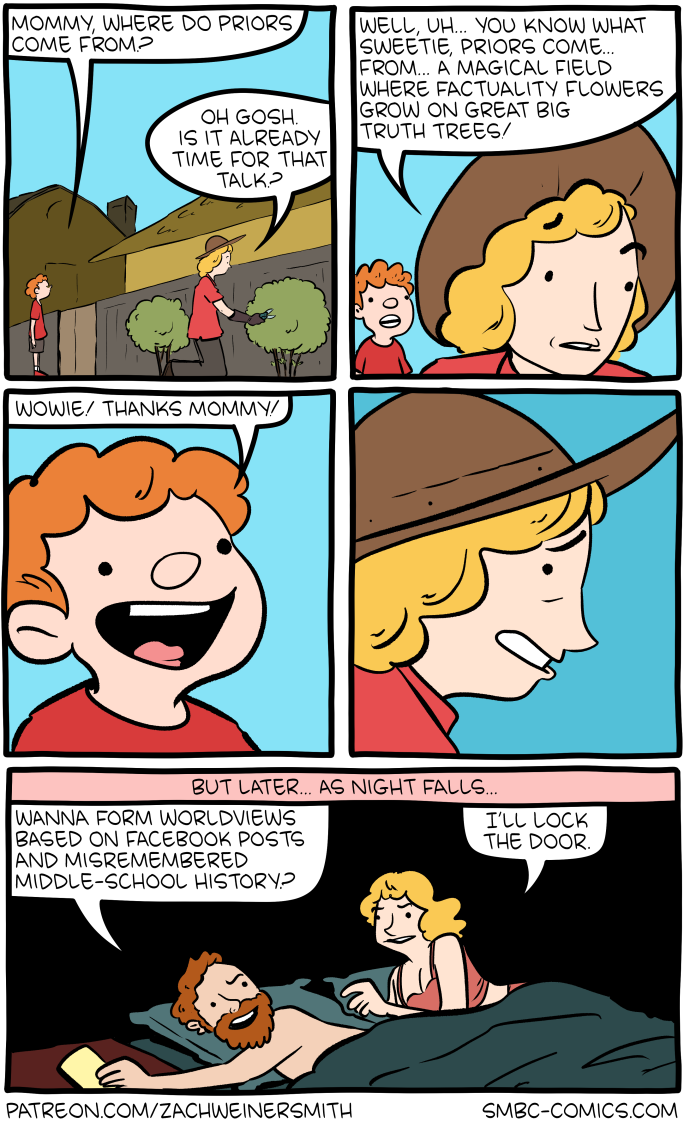
\includegraphics[trim=0 0 0 770,clip,width=6 cm]{Figures/SMBC_1759360612-20251002_priors.png}
\end{figure}
\end{frame}


\begin{frame}{Prior distributions and subjectivity}
\begin{witemize}
\item There is a large discussion about the ``subjectivity'' of priors \parencite[e.g.][]{Berger2006}
\item We will abstract from the philosophical issues arising here
\item Necessarily subjective choices like e.g.\ the model used tend to be more important than the prior over parameters
\item But be aware: issue is contentious as ``subjectivity'' does not square well with the ``scientific method''
\end{witemize}
\end{frame}


\begin{frame}{First things first: Specifying the prior}
\begin{witemize}
\item We need to specify the prior distribution $p(\theta)$
\item In general, this can be a full multivariate distribution
\item In practice, people typically use \highlight{independent priors} \parencite[][is a notable exception]{AndrleBenes2013}
\item Choosing sensible priors is hard, see \textcite{DelNegroetal2008}
\item What is the purpose of priors?
\begin{enumerate}
  \item Incorporating information extraneous to the sample
  \item Providing additional curvature to the likelihood function and straightening out cliffs
\end{enumerate}
\item Parameter range often narrows down prior choice
\item After choosing the priors, you should do a \highlight{prior predictive}: check what the prior implies for the question you are asking \parencite[see][]{LeeperWalkerTraum2017AER}
\item This way, you make sure that your estimation results are not solely driven by your prior
\end{witemize}
\end{frame}

\renewcommand{\Source}{}
\begin{frame}{Endogenous priors}
\begin{witemize}
\item We are doing \highlight{full information} estimation
\item We are not matching moments!
\item Regularly happens that estimated model implies too high variances
\item Proposed solution: \highlight{endogenous priors} \parencite{ChristianoTrabandtWalentin2011,DelNegroetal2008}
\item Motivated by sequential Bayesian learning
\item Starting from independent initial priors, use standard deviations observed in a ``pre-sample'' to update those initial priors.
\item Product of the initial priors and the pre-sample likelihood of the standard deviations of
the observables is used as the new prior
\item Triggered by the \texttt{endogenous\_prior}-option of the Dynare \texttt{estimation}-command
\end{witemize}
\end{frame}

\subsection{Normal Distribution}
\begin{frame}{Normal prior}
\begin{figure}
  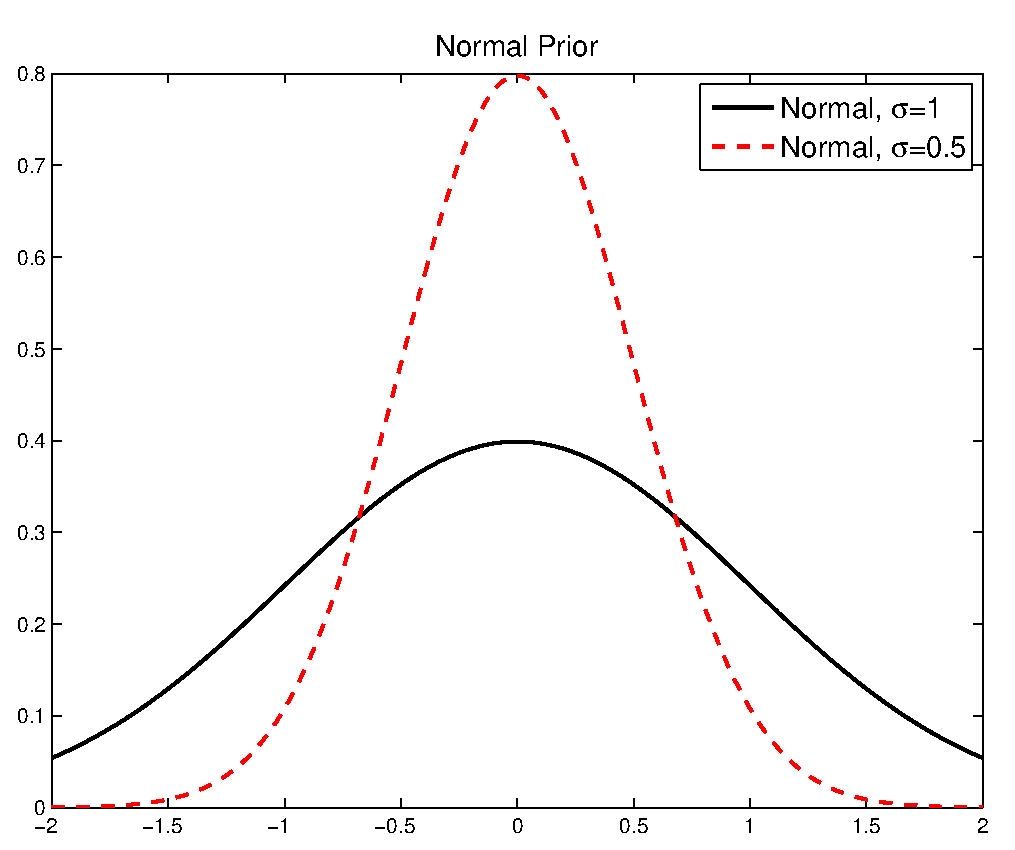
\includegraphics[scale=.45]{Figures/normal_prior}
\end{figure}
\begin{itemize}
\item Unbounded support $(-\infty,\infty)$ and symmetric
\item Typically used for e.g.\ feedback parameters where sign is unknown
\end{itemize}
\end{frame}

\subsection{Uniform Distribution}
\begin{frame}{Uniform prior}
\begin{figure}
  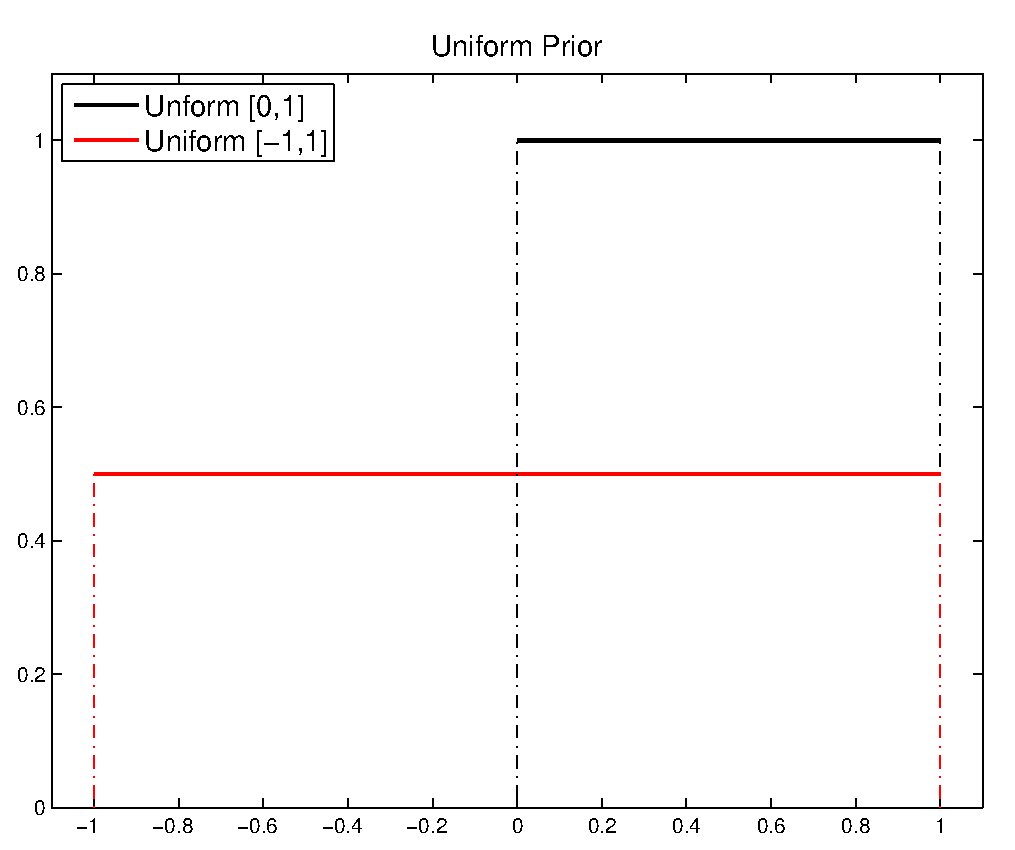
\includegraphics[scale=.45]{Figures/uniform_prior}
\end{figure}
\begin{itemize}
\item Bounded support on $[LB,UB]$
\end{itemize}
\end{frame}

\begin{frame}{Uniform prior}
\begin{itemize}
\item For a variable $Y \sim U(a,b)$, the PDF is given by
    \begin{equation}
    {f_U}\left( {y|a,b} \right) = \left\{ {\begin{array}{*{20}{c}}
      {\frac{1}{{b - a}} \text{ if } a \leqslant y \leqslant b} \\
      {0 \text{ otherwise} }
    \end{array}} \right.
    \end{equation}
    where $-\infty<a<b<\infty $
    \item Moreover,
    \begin{align}
  E\left( Y \right) = \frac{a+b}{2} \hfill \\
  \operatorname{var} \left( Y \right) = \frac{{{{\left( {b - a} \right)}^2}}}{{12}}
\end{align}
    \item Prior is ``flat'', i.e.\ all points are equally likely, and it does not introduce curvature
    \item Often called \highlight{uninformative prior}
    \item But: it is informative in the sense that you say all parameter values in the interval are equally likely
    \item Beware: with bounds at infinity, prior is \highlight{improper} (cf. model comparison)
\end{itemize}
\end{frame}


\subsection{Beta Distribution}
\begin{frame}{Beta prior}
\begin{figure}
  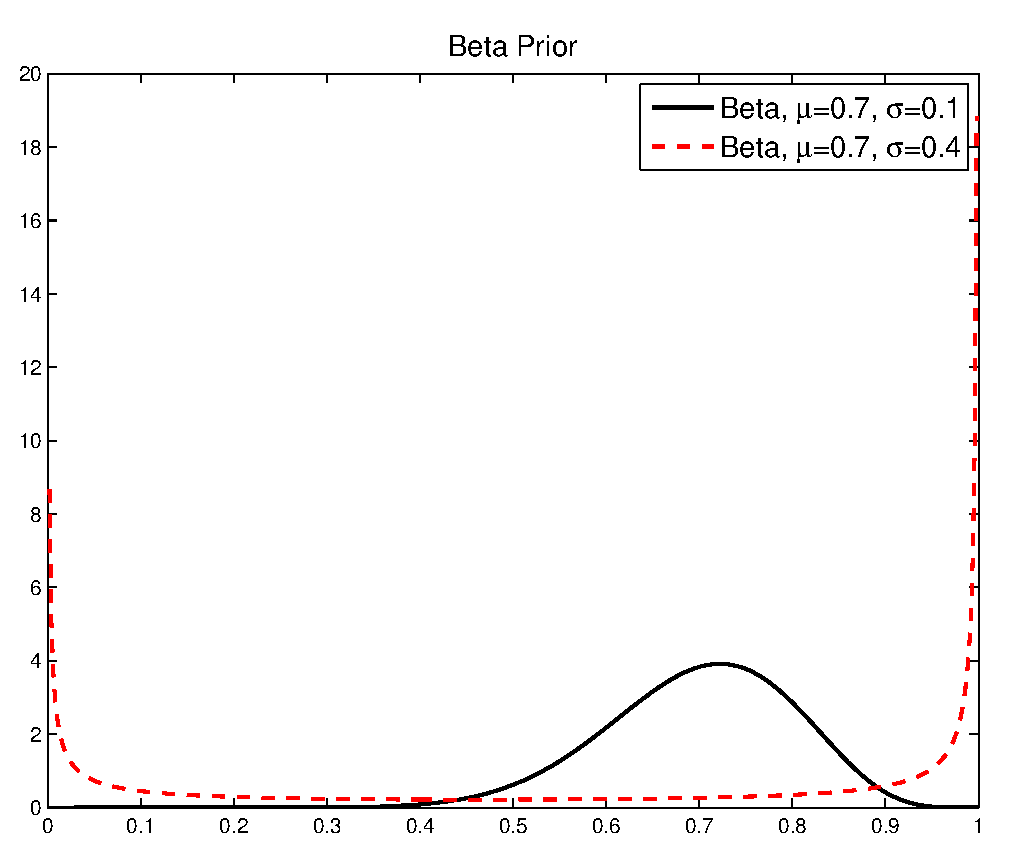
\includegraphics[scale=.45]{Figures/beta_prior}
\end{figure}
\begin{itemize}
\item Bounded support on $[0,1]$
\item Often used for autoregressive parameters, the discount factor, Calvo parameters, etc.
\end{itemize}
\end{frame}

\begin{frame}{Beta prior}
\begin{witemize}
    \item Suitable transformations allow scaling it to different support like $[-1,1]$
    \item Relatively flexible in allowing for different shapes, but care is required
    \item Due to bounded support, a high variance can result in assigning high mass to extremes in the tails
    \item[$\Rightarrow$] mode, i.e.\ point of highest likelihood, far away from prior mean
    \item Always plot the prior distribution!
\end{witemize}
\end{frame}


\subsection{Gamma Distribution}
\begin{frame}{Gamma prior}
\begin{figure}
  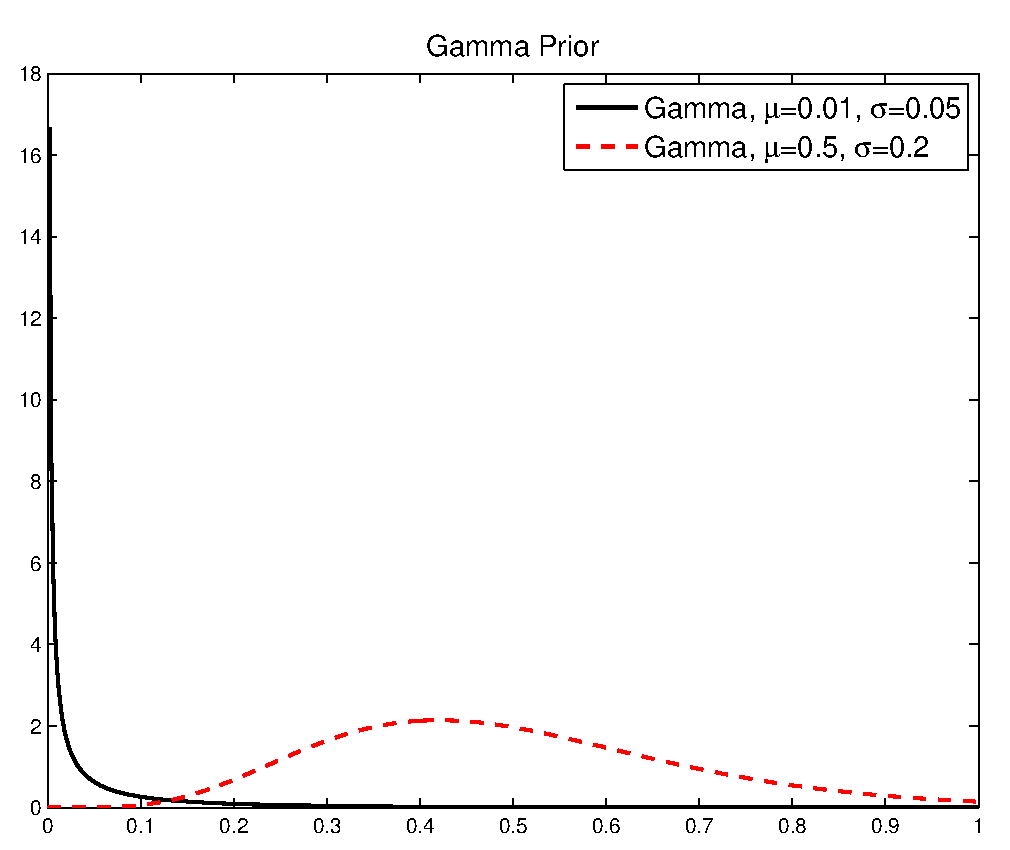
\includegraphics[scale=.45]{Figures/gamma_prior}
\end{figure}
\begin{itemize}
\item Support $[0,\infty)$, i.e.\ 0 is included
\item Typically used for variances and Taylor rule feedback parameters
\end{itemize}
\end{frame}

\begin{frame}{Gamma prior}
\begin{itemize}
\item For a variable $Y \sim G(\mu,\nu)$, where $\mu$ is the mean and $\nu$ the degrees of freedom, the PDF is given by
\begin{equation}
{f_G}\left( {y|\mu,\nu} \right) = \left\{ {\begin{array}{*{20}{c}}
  {\frac{1}{{{{\left( {\frac{{2\mu }}{\nu }} \right)}^{\frac{\nu }{2}}}\Gamma \left( {\frac{\nu }{2}} \right)}}{y^{\frac{{\nu  - 2}}{2}}}{e^{ - \frac{{y\nu }}{{2\mu }}}} \text{ if }0 \leqslant y \leqslant \infty } \\
  {0\text{ otherwise} }
\end{array}} \right. \: ,
\end{equation}
    where $\Gamma()$ is the Gamma function
    \item Moreover,
    \begin{align}
  E\left( Y \right) &= \mu  \hfill \\
  \operatorname{var} \left( Y \right) &= \frac{{2{\mu ^2}}}{\nu }
\end{align}
    \item Beware: Matlab uses ${f_G}\left( {y|a,b} \right)$ with $a = \frac{\nu }{2},b = \frac{{2\mu }}{\nu }$
    \item Thus, use \vspace{-.3cm}
    \begin{align}
  a &= \frac{{{\mu ^2}}}{{{\sigma ^2}}} \hfill \\
  b &= \frac{{{\sigma ^2}}}{\mu }
    \end{align}
\end{itemize}
\end{frame}

\subsection{Inverse Gamma Distribution}
\renewcommand{\Source}{Wikipedia}
\begin{frame}{Inverse Gamma prior}
\begin{figure}
  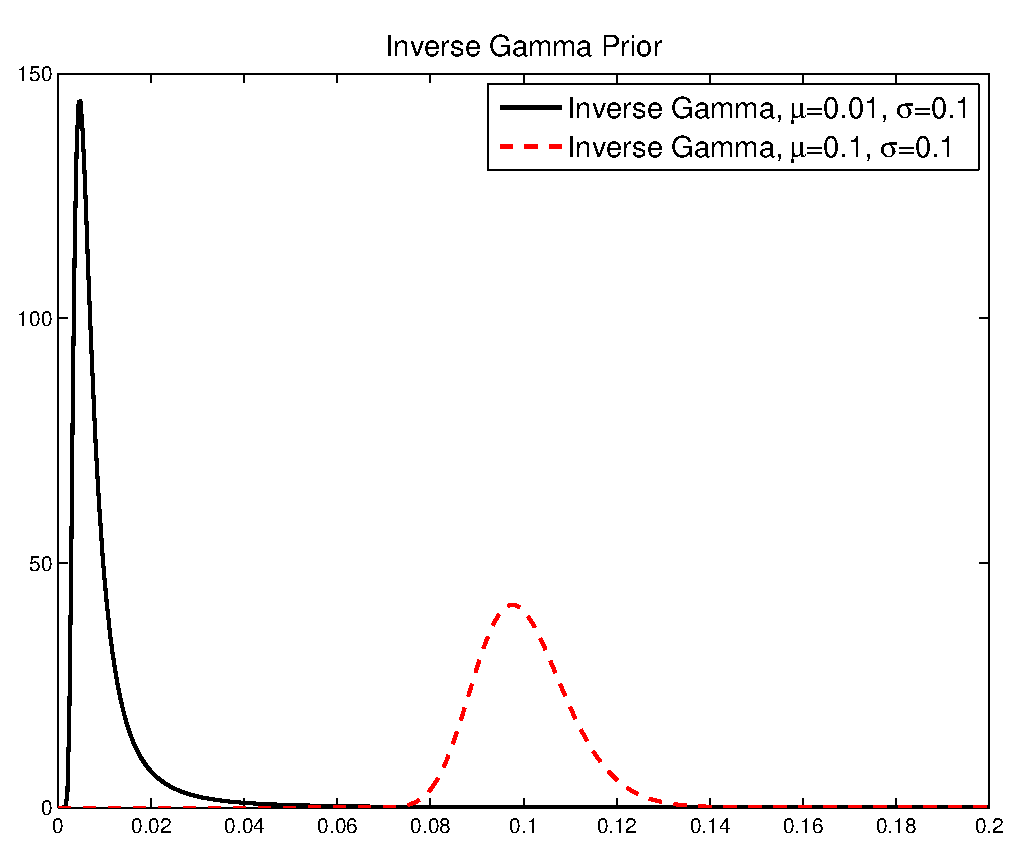
\includegraphics[scale=.45]{Figures/inverse_gamma_prior}
\end{figure}
\begin{itemize}
\item Support $(0,\infty)$, i.e.\ 0 is not included
\item Typically used for variances
\end{itemize}
\end{frame}

\begin{frame}{Inverse Gamma prior}
\begin{itemize}
    \item If $y$ is Inverse Gamma, then $1/y$ is Gamma distributed
    \item The pdf is given by
    \begin{equation}
    {f_{IG}}\left( {y|a,b} \right) = \left\{ {\begin{array}{*{20}{c}}
  {\frac{{{b^a}}}{{\Gamma \left( a \right)}}{y^{a - 1}}{e^{ - by}} \text{ if } 0 \leqslant y \leqslant \infty } \\
  {0 \text{ otherwise} }
\end{array}} \right.
\end{equation}
with
\begin{align}
  E\left( Y \right) &= \frac{a}{b} \hfill \\
  \operatorname{var} \left( Y \right) &= \frac{a}{{{b^2}}}
\end{align}
\item Thus:
    \begin{align}
  a &= \frac{{{\mu ^2}}}{{{\sigma ^2}}} \hfill \\
  b &= \frac{\mu }{{{\sigma ^2}}}
    \end{align}
    \item Theoretically, a better choice for variances  if you want to prevent \highlight{stochastic singularity}
    \item But: variance of exactly 0 is a zero probability event
    \item[$\Rightarrow$] Difference not really important
\end{itemize}
\end{frame}

\subsection{Example}
\renewcommand{\Source}{}
\begin{frame}{Prior plots}{\texttt{\texttt{RBC\_Bayesian.mod}}}
\begin{figure}
  \includegraphics[scale=.65]{Bayesian_Estimation/RBC_Bayesian_Priors1}
\end{figure}
\begin{itemize}
\item Always check whether your prior looks sensible
\end{itemize}
\end{frame}

\begin{frame}{Mode check plots}{\texttt{\texttt{RBC\_Bayesian.mod}}}
\begin{figure}
  \includegraphics[scale=.6]{Bayesian_Estimation/RBC_Bayesian_CheckPlots1}
\end{figure}
\begin{itemize}
\item Notice how the prior affects the posterior for \texttt{rhog}
\end{itemize}
\end{frame}

\section[M-H]{The Metropolis-Hastings algorithm}

\begin{frame}{The problem: drawing from the posterior}

\begin{witemize}
\item We would like to compute
    \begin{equation}
    E\left( {g\left( \theta  \right)|{y^T}} \right) = \int {g\left( \theta  \right)p\left( {\theta |{y^T}} \right)d\theta }  \approx \frac{1}{S}\sum\limits_{s = 1}^S {g\left( {{\theta _s}} \right)} =\hat g_S
    \end{equation}
\item While we can evaluate $p\left( \theta|{y^T}\right)$, we do not know how to draw from it
\item Idea: find mechanism that
\begin{enumerate}
  \item draws from a stand-in proposal density
  \item evaluates both proposal density and target density
  \item reweights the draws based on the comparison of densities to obtain draws from target
\end{enumerate}
\end{witemize}
\end{frame}

\begin{frame}{Metropolis Hastings-algorithm}
\begin{itemize}
    \item Start with a vector $\theta_0$
    \item Repeat for $j=1,\ldots,N$
    \begin{itemize}
        \item Generate candidate $\tilde \theta$ from proposal density $q(\theta_{j-1},\tilde \theta)$ and $u$ from $\mathcal{U}(0,1)$
        \item If $\tilde \theta$ is valid parameter draw (steady state exists, Blanchard-Kahn conditions satisfied etc.) and $u<\alpha(\theta^{j-1},\theta^{j})$ with
        \begin{equation}
        \alpha \left( {\theta_{j-1},\tilde \theta} \right) = \left\{ {\begin{array}{*{20}{c}}
            {\min \left[ {\frac{{p \left( \tilde \theta | y^T\right)q\left( {\tilde \theta,\theta_{j-1}} \right)}}{{p \left(\theta_{j-1} | y^T\right)q\left( {\theta_{j-1},\tilde \theta} \right)}},1} \right] \text{ if }p \left( \theta_{j-1} \right)q\left( {\theta_{j-1},\tilde \theta} \right) > 0} \\
            {1 \text{ otherwise} }
            \end{array}} \right.
        \end{equation}
        set $\theta_j=\tilde \theta$
        \item Otherwise, set $\theta_j=\theta_{j-1}$ (implies setting $p(\tilde \theta)=0$ if draw invalid)
    \end{itemize}
    \item Return the values $\{\theta_0,\ldots,\theta_N\}$
    \item After the chain has passed the \highlight{transient stage} and the effect of the starting values has subsided, the subsequent draws can be considered draws from the posterior
    \item[$\Rightarrow$] \highlight{burn-in} required that assures remaining chain has \highlight{converged}
\end{itemize}
\end{frame}


\begin{frame}{Intuition}
\begin{witemize}
    \item Note: with symmetric density, the scaling probability simplifies to
    \begin{equation}
        \alpha \left( {{\theta _{j - 1}},\tilde \theta} \right) = \min \left[ {\frac{{L\left( {\left. {{Y^T}} \right|\tilde \theta} \right)p\left( \tilde \theta \right)}}{{L\left( {\left. {{Y^T}} \right|{\theta _{j - 1}}} \right)p\left( {{\theta _{j - 1}}} \right)}},1} \right]
    \end{equation}
    \item Jump always ``uphill'' and ``downhill'' with some probability (cf. Simulated Annealing)
\end{witemize}
\end{frame}

\begin{frame}{MH with symmetric proposal: uphill}
  \bigskip
  \begin{center}
  \scalebox{.7}{% This file was created by matlab2tikz.
%
%The latest updates can be retrieved from
%  http://www.mathworks.com/matlabcentral/fileexchange/22022-matlab2tikz-matlab2tikz
%where you can also make suggestions and rate matlab2tikz.
%
\begin{tikzpicture}

\begin{axis}[%
width=4.521in,
height=3.566in,
at={(0.758in,0.481in)},
scale only axis,
clip=false,
xmin=-3.5,
xmax=3.5,
xtick={\empty},
ymin=0,
ymax=0.45,
ytick={\empty},
axis background/.style={fill=white}
]
\addplot [color=black,solid,line width=2.0pt,forget plot]
  table[row sep=crcr]{%
-3.5	0.00087268269504576\\
-3.49	0.000903722211277524\\
-3.48	0.00093577215692748\\
-3.47	0.000968861842919846\\
-3.46	0.00100302130073424\\
-3.45	0.00103828129566141\\
-3.44	0.00107467334015374\\
-3.43	0.00111222970726556\\
-3.42	0.00115098344417848\\
-3.41	0.00119096838580612\\
-3.4	0.00123221916847302\\
-3.39	0.00127477124366183\\
-3.38	0.00131866089182274\\
-3.37	0.0013639252362389\\
-3.36	0.00141060225694139\\
-3.35	0.00145873080466675\\
-3.34	0.00150835061485031\\
-3.33	0.00155950232164769\\
-3.32	0.00161222747197712\\
-3.31	0.00166656853957458\\
-3.3	0.00172256893905368\\
-3.29	0.00178027303996188\\
-3.28	0.00183972618082428\\
-3.27	0.00190097468316608\\
-3.26	0.00196406586550438\\
-3.25	0.00202904805729977\\
-3.24	0.00209597061285794\\
-3.23	0.00216488392517106\\
-3.22	0.00223583943968854\\
-3.21	0.0023088896680065\\
-3.2	0.00238408820146484\\
-3.19	0.0024614897246407\\
-3.18	0.00254115002872652\\
-3.17	0.00262312602478102\\
-3.16	0.0027074757568407\\
-3.15	0.00279425841487945\\
-3.14	0.00288353434760344\\
-3.13	0.00297536507506825\\
-3.12	0.00306981330110474\\
-3.11	0.00316694292554008\\
-3.1	0.00326681905619992\\
-3.09	0.00336950802067748\\
-3.08	0.00347507737785494\\
-3.07	0.00358359592916236\\
-3.06	0.00369513372955903\\
-3.05	0.00380976209822181\\
-3.04	0.00392755362892478\\
-3.03	0.00404858220009443\\
-3.02	0.00417292298452396\\
-3.01	0.00430065245873045\\
-3	0.00443184841193801\\
-2.99	0.00456658995467015\\
-2.98	0.00470495752693398\\
-2.97	0.00484703290597895\\
-2.96	0.00499289921361238\\
-2.95	0.00514264092305394\\
-2.94	0.00529634386531102\\
-2.93	0.00545409523505656\\
-2.92	0.00561598359599097\\
-2.91	0.00578209888566947\\
-2.9	0.00595253241977585\\
-2.89	0.00612737689582369\\
-2.88	0.00630672639626593\\
-2.87	0.00649067639099336\\
-2.86	0.00667932373920262\\
-2.85	0.00687276669061397\\
-2.84	0.00707110488601945\\
-2.83	0.00727443935714122\\
-2.82	0.00748287252578056\\
-2.81	0.00769650820223732\\
-2.8	0.00791545158297997\\
-2.79	0.00813980924754602\\
-2.78	0.00836968915465302\\
-2.77	0.00860520063749967\\
-2.76	0.00884645439823723\\
-2.75	0.00909356250159105\\
-2.74	0.00934663836761228\\
-2.73	0.00960579676353959\\
-2.72	0.00987115379475115\\
-2.71	0.0101428268947871\\
-2.7	0.0104209348144226\\
-2.69	0.0107055976097722\\
-2.68	0.0109969366294056\\
-2.67	0.0112950745004561\\
-2.66	0.0116001351137026\\
-2.65	0.0119122436076052\\
-2.64	0.012231526351278\\
-2.63	0.0125581109263782\\
-2.62	0.0128921261078953\\
-2.61	0.0132337018438214\\
-2.6	0.0135829692336856\\
-2.59	0.0139400605059358\\
-2.58	0.0143051089941497\\
-2.57	0.01467824911206\\
-2.56	0.0150596163273774\\
-2.55	0.0154493471343952\\
-2.54	0.0158475790253608\\
-2.53	0.0162544504606005\\
-2.52	0.0166701008373811\\
-2.51	0.017094670457497\\
-2.5	0.0175283004935685\\
-2.49	0.0179711329540396\\
-2.48	0.018423310646862\\
-2.47	0.0188849771418562\\
-2.46	0.019356276731737\\
-2.45	0.0198373543917953\\
-2.44	0.0203283557382258\\
-2.43	0.0208294269850922\\
-2.42	0.0213407148999228\\
-2.41	0.0218623667579294\\
-2.4	0.0223945302948429\\
-2.39	0.0229373536583607\\
-2.38	0.0234909853582014\\
-2.37	0.024055574214763\\
-2.36	0.0246312693063825\\
-2.35	0.0252182199151944\\
-2.34	0.0258165754715877\\
-2.33	0.0264264854972617\\
-2.32	0.0270480995468818\\
-2.31	0.0276815671483366\\
-2.3	0.0283270377416012\\
-2.29	0.0289846606162094\\
-2.28	0.0296545848473413\\
-2.27	0.0303369592305316\\
-2.26	0.0310319322150083\\
-2.25	0.0317396518356674\\
-2.24	0.0324602656436974\\
-2.23	0.0331939206358611\\
-2.22	0.0339407631824492\\
-2.21	0.0347009389539188\\
-2.2	0.0354745928462314\\
-2.19	0.0362618689049062\\
-2.18	0.0370629102478065\\
-2.17	0.0378778589866775\\
-2.16	0.0387068561474556\\
-2.15	0.0395500415893702\\
-2.14	0.0404075539228603\\
-2.13	0.0412795304263304\\
-2.12	0.0421661069617703\\
-2.11	0.0430674178892657\\
-2.1	0.0439835959804272\\
-2.09	0.0449147723307671\\
-2.08	0.0458610762710549\\
-2.07	0.0468226352776831\\
-2.06	0.047799574882077\\
-2.05	0.0487920185791828\\
-2.04	0.0498000877350708\\
-2.03	0.0508239014936912\\
-2.02	0.0518635766828206\\
-2.01	0.0529192277192403\\
-2	0.0539909665131881\\
-1.99	0.0550789023721258\\
-1.98	0.056183141903868\\
-1.97	0.0573037889191171\\
-1.96	0.0584409443334515\\
-1.95	0.0595947060688161\\
-1.94	0.0607651689545648\\
-1.93	0.0619524246281052\\
-1.92	0.0631565614351987\\
-1.91	0.0643776643299694\\
-1.9	0.0656158147746766\\
-1.89	0.0668710906393072\\
-1.88	0.0681435661010446\\
-1.87	0.0694333115436742\\
-1.86	0.0707403934569834\\
-1.85	0.072064874336218\\
-1.84	0.0734068125816569\\
-1.83	0.0747662623983676\\
-1.82	0.0761432736962073\\
-1.81	0.077537891990134\\
-1.8	0.0789501583008941\\
-1.79	0.0803801090561542\\
-1.78	0.0818277759921428\\
-1.77	0.0832931860558745\\
-1.76	0.0847763613080222\\
-1.75	0.0862773188265115\\
-1.74	0.0877960706109056\\
-1.73	0.089332623487655\\
-1.72	0.0908869790162829\\
-1.71	0.0924591333965807\\
-1.7	0.0940490773768869\\
-1.69	0.095656796163524\\
-1.68	0.0972822693314675\\
-1.67	0.0989254707363237\\
-1.66	0.100586368427691\\
-1.65	0.102264924563978\\
-1.64	0.103961095328764\\
-1.63	0.105674830848764\\
-1.62	0.107406075113484\\
-1.61	0.109154765896647\\
-1.6	0.110920834679456\\
-1.59	0.112704206575771\\
-1.58	0.114504800259292\\
-1.57	0.116322527892807\\
-1.56	0.118157295059582\\
-1.55	0.120009000696986\\
-1.54	0.121877537032402\\
-1.53	0.123762789521523\\
-1.52	0.125664636789088\\
-1.51	0.127582950572142\\
-1.5	0.129517595665892\\
-1.49	0.131468429872231\\
-1.48	0.133435303951002\\
-1.47	0.135418061574071\\
-1.46	0.137416539282282\\
-1.45	0.13943056644536\\
-1.44	0.141459965224839\\
-1.43	0.143504550540062\\
-1.42	0.145564130037348\\
-1.41	0.147638504062356\\
-1.4	0.149727465635745\\
-1.39	0.151830800432162\\
-1.38	0.153948286762634\\
-1.37	0.156079695560421\\
-1.36	0.158224790370383\\
-1.35	0.16038332734192\\
-1.34	0.162555055225534\\
-1.33	0.164739715373077\\
-1.32	0.166937041741714\\
-1.31	0.169146760901672\\
-1.3	0.171368592047807\\
-1.29	0.173602247015033\\
-1.28	0.175847430297662\\
-1.27	0.178103839072694\\
-1.26	0.18037116322708\\
-1.25	0.182649085389022\\
-1.24	0.184937280963305\\
-1.23	0.18723541817073\\
-1.22	0.18954315809164\\
-1.21	0.191860154713599\\
-1.2	0.194186054983213\\
-1.19	0.196520498862137\\
-1.18	0.198863119387276\\
-1.17	0.201213542735197\\
-1.16	0.203571388290759\\
-1.15	0.205936268719975\\
-1.14	0.208307790047108\\
-1.13	0.210685551736015\\
-1.12	0.213069146775718\\
-1.11	0.21545816177022\\
-1.1	0.217852177032551\\
-1.09	0.220250766683033\\
-1.08	0.222653498751761\\
-1.07	0.22505993528527\\
-1.06	0.227469632457386\\
-1.05	0.229882140684233\\
-1.04	0.232297004743366\\
-1.03	0.234713763897012\\
-1.02	0.23713195201938\\
-1.01	0.239551097728013\\
-1	0.241970724519143\\
-0.99	0.244390350907\\
-0.98	0.246809490567043\\
-0.97	0.249227652483066\\
-0.96	0.251644341098117\\
-0.95	0.254059056469189\\
-0.94	0.25647129442562\\
-0.93	0.258880546731149\\
-0.92	0.261286301249553\\
-0.91	0.263688042113818\\
-0.9	0.266085249898755\\
-0.89	0.268477401797002\\
-0.88	0.270863971798338\\
-0.87	0.273244430872216\\
-0.86	0.275618247153457\\
-0.85	0.277984886130996\\
-0.84	0.280343810839621\\
-0.83	0.28269448205458\\
-0.82	0.285036358489007\\
-0.81	0.287368896994028\\
-0.8	0.289691552761483\\
-0.79	0.292003779529141\\
-0.78	0.294305029788325\\
-0.77	0.296594754993816\\
-0.76	0.298872405775953\\
-0.75	0.301137432154804\\
-0.74	0.3033892837563\\
-0.73	0.30562741003021\\
-0.72	0.307851260469853\\
-0.71	0.310060284833416\\
-0.7	0.312253933366761\\
-0.69	0.314431657027597\\
-0.68	0.316592907710893\\
-0.67	0.318737138475402\\
-0.66	0.320863803771172\\
-0.65	0.322972359667914\\
-0.64	0.325062264084082\\
-0.63	0.327132977016555\\
-0.62	0.329183960770765\\
-0.61	0.331214680191153\\
-0.6	0.3332246028918\\
-0.59	0.335213199487106\\
-0.58	0.337179943822381\\
-0.57	0.339124313204192\\
-0.56	0.341045788630353\\
-0.55	0.342943855019384\\
-0.54	0.344818001439333\\
-0.53	0.346667721335792\\
-0.52	0.348492512758975\\
-0.51	0.350291878589726\\
-0.5	0.3520653267643\\
-0.49	0.35381237049778\\
-0.48	0.355532528505997\\
-0.47	0.357225325225801\\
-0.46	0.358890291033545\\
-0.45	0.360526962461648\\
-0.44	0.362134882413092\\
-0.43	0.363713600373713\\
-0.42	0.365262672622154\\
-0.41	0.366781662437336\\
-0.4	0.368270140303323\\
-0.39	0.369727684111432\\
-0.38	0.371153879359466\\
-0.37	0.372548319347933\\
-0.36	0.373910605373128\\
-0.35	0.375240346916938\\
-0.34	0.376537161833254\\
-0.33	0.377800676530865\\
-0.32	0.379030526152702\\
-0.31	0.380226354751325\\
-0.3	0.381387815460524\\
-0.29	0.382514570662924\\
-0.28	0.383606292153479\\
-0.27	0.384662661298743\\
-0.26	0.385683369191816\\
-0.25	0.386668116802849\\
-0.24	0.387616615125014\\
-0.23	0.388528585315836\\
-0.22	0.38940375883379\\
-0.21	0.390241877570074\\
-0.2	0.391042693975456\\
-0.19	0.391805971182121\\
-0.18	0.392531483120429\\
-0.17	0.393219014630497\\
-0.16	0.393868361568541\\
-0.15	0.394479330907889\\
-0.14	0.395051740834611\\
-0.13	0.395585420837687\\
-0.12	0.396080211793656\\
-0.11	0.396535966045686\\
-0.1	0.396952547477012\\
-0.0899999999999999	0.397329831578688\\
-0.0800000000000001	0.397667705511609\\
-0.0699999999999998	0.397966068162751\\
-0.0600000000000001	0.398224830195607\\
-0.0499999999999998	0.398443914094764\\
-0.04	0.398623254204605\\
-0.0299999999999998	0.3987627967621\\
-0.02	0.398862499923666\\
-0.00999999999999979	0.398922333786082\\
0	0.398942280401433\\
0.00999999999999979	0.398922333786082\\
0.02	0.398862499923666\\
0.0299999999999998	0.3987627967621\\
0.04	0.398623254204605\\
0.0499999999999998	0.398443914094764\\
0.0600000000000001	0.398224830195607\\
0.0699999999999998	0.397966068162751\\
0.0800000000000001	0.397667705511609\\
0.0899999999999999	0.397329831578688\\
0.1	0.396952547477012\\
0.11	0.396535966045686\\
0.12	0.396080211793656\\
0.13	0.395585420837687\\
0.14	0.395051740834611\\
0.15	0.394479330907889\\
0.16	0.393868361568541\\
0.17	0.393219014630497\\
0.18	0.392531483120429\\
0.19	0.391805971182121\\
0.2	0.391042693975456\\
0.21	0.390241877570074\\
0.22	0.38940375883379\\
0.23	0.388528585315836\\
0.24	0.387616615125014\\
0.25	0.386668116802849\\
0.26	0.385683369191816\\
0.27	0.384662661298743\\
0.28	0.383606292153479\\
0.29	0.382514570662924\\
0.3	0.381387815460524\\
0.31	0.380226354751325\\
0.32	0.379030526152702\\
0.33	0.377800676530865\\
0.34	0.376537161833254\\
0.35	0.375240346916938\\
0.36	0.373910605373128\\
0.37	0.372548319347933\\
0.38	0.371153879359466\\
0.39	0.369727684111432\\
0.4	0.368270140303323\\
0.41	0.366781662437336\\
0.42	0.365262672622154\\
0.43	0.363713600373713\\
0.44	0.362134882413092\\
0.45	0.360526962461648\\
0.46	0.358890291033545\\
0.47	0.357225325225801\\
0.48	0.355532528505997\\
0.49	0.35381237049778\\
0.5	0.3520653267643\\
0.51	0.350291878589726\\
0.52	0.348492512758975\\
0.53	0.346667721335792\\
0.54	0.344818001439333\\
0.55	0.342943855019384\\
0.56	0.341045788630353\\
0.57	0.339124313204192\\
0.58	0.337179943822381\\
0.59	0.335213199487106\\
0.6	0.3332246028918\\
0.61	0.331214680191153\\
0.62	0.329183960770765\\
0.63	0.327132977016555\\
0.64	0.325062264084082\\
0.65	0.322972359667914\\
0.66	0.320863803771172\\
0.67	0.318737138475402\\
0.68	0.316592907710893\\
0.69	0.314431657027597\\
0.7	0.312253933366761\\
0.71	0.310060284833416\\
0.72	0.307851260469853\\
0.73	0.30562741003021\\
0.74	0.3033892837563\\
0.75	0.301137432154804\\
0.76	0.298872405775953\\
0.77	0.296594754993816\\
0.78	0.294305029788325\\
0.79	0.292003779529141\\
0.8	0.289691552761483\\
0.81	0.287368896994028\\
0.82	0.285036358489007\\
0.83	0.28269448205458\\
0.84	0.280343810839621\\
0.85	0.277984886130996\\
0.86	0.275618247153457\\
0.87	0.273244430872216\\
0.88	0.270863971798338\\
0.89	0.268477401797002\\
0.9	0.266085249898755\\
0.91	0.263688042113818\\
0.92	0.261286301249553\\
0.93	0.258880546731149\\
0.94	0.25647129442562\\
0.95	0.254059056469189\\
0.96	0.251644341098117\\
0.97	0.249227652483066\\
0.98	0.246809490567043\\
0.99	0.244390350907\\
1	0.241970724519143\\
1.01	0.239551097728013\\
1.02	0.23713195201938\\
1.03	0.234713763897012\\
1.04	0.232297004743366\\
1.05	0.229882140684233\\
1.06	0.227469632457386\\
1.07	0.22505993528527\\
1.08	0.222653498751761\\
1.09	0.220250766683033\\
1.1	0.217852177032551\\
1.11	0.21545816177022\\
1.12	0.213069146775718\\
1.13	0.210685551736015\\
1.14	0.208307790047108\\
1.15	0.205936268719975\\
1.16	0.203571388290759\\
1.17	0.201213542735197\\
1.18	0.198863119387276\\
1.19	0.196520498862137\\
1.2	0.194186054983213\\
1.21	0.191860154713599\\
1.22	0.18954315809164\\
1.23	0.18723541817073\\
1.24	0.184937280963305\\
1.25	0.182649085389022\\
1.26	0.18037116322708\\
1.27	0.178103839072694\\
1.28	0.175847430297662\\
1.29	0.173602247015033\\
1.3	0.171368592047807\\
1.31	0.169146760901672\\
1.32	0.166937041741714\\
1.33	0.164739715373077\\
1.34	0.162555055225534\\
1.35	0.16038332734192\\
1.36	0.158224790370383\\
1.37	0.156079695560421\\
1.38	0.153948286762634\\
1.39	0.151830800432162\\
1.4	0.149727465635745\\
1.41	0.147638504062356\\
1.42	0.145564130037348\\
1.43	0.143504550540062\\
1.44	0.141459965224839\\
1.45	0.13943056644536\\
1.46	0.137416539282282\\
1.47	0.135418061574071\\
1.48	0.133435303951002\\
1.49	0.131468429872231\\
1.5	0.129517595665892\\
1.51	0.127582950572142\\
1.52	0.125664636789088\\
1.53	0.123762789521523\\
1.54	0.121877537032402\\
1.55	0.120009000696986\\
1.56	0.118157295059582\\
1.57	0.116322527892807\\
1.58	0.114504800259292\\
1.59	0.112704206575771\\
1.6	0.110920834679456\\
1.61	0.109154765896647\\
1.62	0.107406075113484\\
1.63	0.105674830848764\\
1.64	0.103961095328764\\
1.65	0.102264924563978\\
1.66	0.100586368427691\\
1.67	0.0989254707363237\\
1.68	0.0972822693314675\\
1.69	0.095656796163524\\
1.7	0.0940490773768869\\
1.71	0.0924591333965807\\
1.72	0.0908869790162829\\
1.73	0.089332623487655\\
1.74	0.0877960706109056\\
1.75	0.0862773188265115\\
1.76	0.0847763613080222\\
1.77	0.0832931860558745\\
1.78	0.0818277759921428\\
1.79	0.0803801090561542\\
1.8	0.0789501583008941\\
1.81	0.077537891990134\\
1.82	0.0761432736962073\\
1.83	0.0747662623983676\\
1.84	0.0734068125816569\\
1.85	0.072064874336218\\
1.86	0.0707403934569834\\
1.87	0.0694333115436742\\
1.88	0.0681435661010446\\
1.89	0.0668710906393072\\
1.9	0.0656158147746766\\
1.91	0.0643776643299694\\
1.92	0.0631565614351987\\
1.93	0.0619524246281052\\
1.94	0.0607651689545648\\
1.95	0.0595947060688161\\
1.96	0.0584409443334515\\
1.97	0.0573037889191171\\
1.98	0.056183141903868\\
1.99	0.0550789023721258\\
2	0.0539909665131881\\
2.01	0.0529192277192403\\
2.02	0.0518635766828206\\
2.03	0.0508239014936912\\
2.04	0.0498000877350708\\
2.05	0.0487920185791828\\
2.06	0.047799574882077\\
2.07	0.0468226352776831\\
2.08	0.0458610762710549\\
2.09	0.0449147723307671\\
2.1	0.0439835959804272\\
2.11	0.0430674178892657\\
2.12	0.0421661069617703\\
2.13	0.0412795304263304\\
2.14	0.0404075539228603\\
2.15	0.0395500415893702\\
2.16	0.0387068561474556\\
2.17	0.0378778589866775\\
2.18	0.0370629102478065\\
2.19	0.0362618689049062\\
2.2	0.0354745928462314\\
2.21	0.0347009389539188\\
2.22	0.0339407631824492\\
2.23	0.0331939206358611\\
2.24	0.0324602656436974\\
2.25	0.0317396518356674\\
2.26	0.0310319322150083\\
2.27	0.0303369592305316\\
2.28	0.0296545848473413\\
2.29	0.0289846606162094\\
2.3	0.0283270377416012\\
2.31	0.0276815671483366\\
2.32	0.0270480995468818\\
2.33	0.0264264854972617\\
2.34	0.0258165754715877\\
2.35	0.0252182199151944\\
2.36	0.0246312693063825\\
2.37	0.024055574214763\\
2.38	0.0234909853582014\\
2.39	0.0229373536583607\\
2.4	0.0223945302948429\\
2.41	0.0218623667579294\\
2.42	0.0213407148999228\\
2.43	0.0208294269850922\\
2.44	0.0203283557382258\\
2.45	0.0198373543917953\\
2.46	0.019356276731737\\
2.47	0.0188849771418562\\
2.48	0.018423310646862\\
2.49	0.0179711329540396\\
2.5	0.0175283004935685\\
2.51	0.017094670457497\\
2.52	0.0166701008373811\\
2.53	0.0162544504606005\\
2.54	0.0158475790253608\\
2.55	0.0154493471343952\\
2.56	0.0150596163273774\\
2.57	0.01467824911206\\
2.58	0.0143051089941497\\
2.59	0.0139400605059358\\
2.6	0.0135829692336856\\
2.61	0.0132337018438214\\
2.62	0.0128921261078953\\
2.63	0.0125581109263782\\
2.64	0.012231526351278\\
2.65	0.0119122436076052\\
2.66	0.0116001351137026\\
2.67	0.0112950745004561\\
2.68	0.0109969366294056\\
2.69	0.0107055976097722\\
2.7	0.0104209348144226\\
2.71	0.0101428268947871\\
2.72	0.00987115379475115\\
2.73	0.00960579676353959\\
2.74	0.00934663836761228\\
2.75	0.00909356250159105\\
2.76	0.00884645439823723\\
2.77	0.00860520063749967\\
2.78	0.00836968915465302\\
2.79	0.00813980924754602\\
2.8	0.00791545158297997\\
2.81	0.00769650820223732\\
2.82	0.00748287252578056\\
2.83	0.00727443935714122\\
2.84	0.00707110488601945\\
2.85	0.00687276669061397\\
2.86	0.00667932373920262\\
2.87	0.00649067639099336\\
2.88	0.00630672639626593\\
2.89	0.00612737689582369\\
2.9	0.00595253241977585\\
2.91	0.00578209888566947\\
2.92	0.00561598359599097\\
2.93	0.00545409523505656\\
2.94	0.00529634386531102\\
2.95	0.00514264092305394\\
2.96	0.00499289921361238\\
2.97	0.00484703290597895\\
2.98	0.00470495752693398\\
2.99	0.00456658995467015\\
3	0.00443184841193801\\
3.01	0.00430065245873045\\
3.02	0.00417292298452396\\
3.03	0.00404858220009443\\
3.04	0.00392755362892478\\
3.05	0.00380976209822181\\
3.06	0.00369513372955903\\
3.07	0.00358359592916236\\
3.08	0.00347507737785494\\
3.09	0.00336950802067748\\
3.1	0.00326681905619992\\
3.11	0.00316694292554008\\
3.12	0.00306981330110474\\
3.13	0.00297536507506825\\
3.14	0.00288353434760344\\
3.15	0.00279425841487945\\
3.16	0.0027074757568407\\
3.17	0.00262312602478102\\
3.18	0.00254115002872652\\
3.19	0.0024614897246407\\
3.2	0.00238408820146484\\
3.21	0.0023088896680065\\
3.22	0.00223583943968854\\
3.23	0.00216488392517106\\
3.24	0.00209597061285794\\
3.25	0.00202904805729977\\
3.26	0.00196406586550438\\
3.27	0.00190097468316608\\
3.28	0.00183972618082428\\
3.29	0.00178027303996188\\
3.3	0.00172256893905368\\
3.31	0.00166656853957458\\
3.32	0.00161222747197712\\
3.33	0.00155950232164769\\
3.34	0.00150835061485031\\
3.35	0.00145873080466675\\
3.36	0.00141060225694139\\
3.37	0.0013639252362389\\
3.38	0.00131866089182274\\
3.39	0.00127477124366183\\
3.4	0.00123221916847302\\
3.41	0.00119096838580612\\
3.42	0.00115098344417848\\
3.43	0.00111222970726556\\
3.44	0.00107467334015374\\
3.45	0.00103828129566141\\
3.46	0.00100302130073424\\
3.47	0.000968861842919846\\
3.48	0.00093577215692748\\
3.49	0.000903722211277524\\
3.5	0.00087268269504576\\
};
\addplot [color=blue,dashed,line width=1.0pt,forget plot]
  table[row sep=crcr]{%
-1	0\\
-1	0.241970724519143\\
};
\addplot [color=red,dashed,line width=1.0pt,forget plot]
  table[row sep=crcr]{%
-0	0\\
-0	0.398942280401433\\
};
\addplot [color=blue,dashed,line width=1.0pt,forget plot]
  table[row sep=crcr]{%
-3.5	0.241970724519143\\
-1	0.241970724519143\\
};
\addplot [color=red,dashed,line width=1.0pt,forget plot]
  table[row sep=crcr]{%
-3.5	0.398942280401433\\
-0	0.398942280401433\\
};
\addplot [color=black,only marks,mark=*,mark options={solid,fill=blue,draw=blue},forget plot]
  table[row sep=crcr]{%
-1	0.241970724519143\\
};
\addplot [color=red,only marks,mark=*,mark options={solid,fill=red,draw=red},forget plot]
  table[row sep=crcr]{%
-0	0.398942280401433\\
};
\node[right, align=left, text=black]
at (axis cs:-1,-0.02) {$ \theta^0  $};
\node[right, align=left, text=black]
at (axis cs:-4.6,0.242) {$  p \left(\theta^0| Y^T\right)  $};
\node[right, align=left, text=black]
at (axis cs:-0.25,-0.02) {$\theta^{1} =  \tilde \theta $};
\node[right, align=left, text=black]
at (axis cs:-4.6,0.399) {$  p \left(\theta^1 | Y^T\right) $};
\node[right, align=left, text=black]
at (axis cs:0,0.419) {$  \alpha=1 $};
\end{axis}
\end{tikzpicture}%}
  \end{center}
\end{frame}


\begin{frame}{MH with symmetric proposal: downhill}
  \bigskip
  \begin{center}
  \scalebox{.7}{\input{Figures/mhplot-c.tex}}
  \end{center}
\end{frame}


\subsection{Choosing a Proposal Density}
\begin{frame}{The Random-Walk Metropolis Hastings algorithm}
\begin{witemize}
    \item As long as the regularity conditions are satisfied, any proposal density $q$ will ultimately lead to convergence to the invariant distribution
    \item However: speed of convergence may differ significantly
    \item In practice, people often use the \highlight{Random-Walk Metropolis Hastings} algorithm where
    \begin{equation}
    q\left( \theta_{j-1},\tilde \theta \right) = {q_{RW}}\left( \theta_{j-1}-\tilde \theta \right)
    \end{equation}
    and $q_{RW}$ is a multivariate density
    \item The candidate $\tilde \theta$ is thus given by the old value $\theta_{j-1}$ plus a random variable increment
    \begin{equation}
    \tilde \theta=\theta_{j-1}+z, z\sim q_{RW}
    \end{equation}
 \end{witemize}
\end{frame}

\begin{frame}{Choosing a proposal density}
\begin{witemize}
    \item Often, one uses
    \begin{equation}
    q_{RW}=\mathcal{N}(0,c^2\Sigma) \text{ or } q_{RW}=t_\nu(0,c^2\Sigma)
    \end{equation}
    \item Thus, one needs a \highlight{scaling matrix} $\Sigma$ and a \highlight{scaling factor} $c$
    \item Idea: construct Gaussian approximation to posterior and use asymptotic covariance matrix as scaling matrix
    \item Allows efficient evaluation around mode
    \item Note: asymptotically, the prior plays no role and the posterior will only depend on the likelihood
    \item \textcite{Koop2003} only uses likelihood function, while \textcite{AnSchorfheide2007} use posterior; we side with the latter
\end{witemize}
\end{frame}

\begin{frame}{Asymptotic normality}
\begin{witemize}
    \item Using normal approximation is justified, because with regularity conditions, posterior of $\theta $ will be \highlight{asymptotically normal} \parencite[see e.g.][]{Walker1969,Kim1998,Crowder1998}
    \item But convergence may be slow
    \item Normal approximation can often be improved by \highlight{natural re-parametrization} \parencite{Adolfsonetal2007}: bring bounded parameters to unbounded support:
    \begin{itemize}
      \item log transformation of positive parameters
      \item logit-transformation for parameters on unit interval
    \end{itemize}

\end{witemize}
\end{frame}

\subsection{The Scaling of the Proposal Density}
\renewcommand{\Source}{}
\begin{frame}{Technical considerations: the starting point}
\begin{witemize}
    \item Usual procedure: use numerical optimizer to find \highlight{posterior mode} of log-posterior $p(\theta|Y^T)$
    \item In practical applications, non-derivative based optimizers seem to perform better
    \item Finding the mode is hard and time-intensive; try (sequence of) different optimizers
    \item In some sense, finding the mode is not important as long as the regularity conditions are met (positive definite scaling matrix)
    \item Wherever you start, asymptotically the MCMC sampler will spend most time at the mode and get there
    \item MCMC is a quite inefficient optimizer (cf. Simulated Annealing)
    \item Thus: if you only have finite time, try to get as close as possible
    \item Problems of not having found the mode can often be seen as a slow drift in the parameters and posterior density
\end{witemize}
\end{frame}

\begin{frame}{Technical considerations: the scaling matrix I}
\begin{witemize}
    \item Set the scaling matrix $\Sigma$ to the \highlight{inverse Hessian} at the posterior mode:
    \begin{equation}
    \Sigma=\operatorname{var} \left( {\hat \theta } \right) = I\left( \theta  \right)^{-1} = {\left( { - E\left[ {\frac{{{\partial ^2}\log p\left( {\theta |Y} \right)}}{{\partial \theta \partial \theta '}}} \right]} \right)^{ - 1}}
    \end{equation}
    \item \texttt{csminwel/newrat} will provide an estimate of the Hessian as one of its outputs
    \item In practice, having fatter tails often works better: might want to use $t$-distribution instead of normal
    \item Sounds easy, but creates a lot of problems!
\end{witemize}
\end{frame}

\begin{frame}{Technical considerations: the scaling matrix II}
\begin{witemize}
    \item Theoretical Inverse Hessian at the true mode is positive definite, but the numerical one at the conjectured mode often is not
    \item Literature uses various (dirty) tricks like
    \begin{witemize}
      \item use Jordan decomposition to decompose matrix, set the eigenvalues smaller than or equal 0 to some small number, and then recompose the matrix
      \item use \highlight{generalized Cholesky} \parencite[see e.g.][]{GillKing2004}
      \item Try different step sizes for numerical evaluation of derivatives \parencite{AnSchorfheide2007}\\
      $\rightarrow$ $\texttt{analytic\_derivation}$-option can also help
    \end{witemize}
\end{witemize}
\end{frame}

\begin{frame}{Non-positive definite Hessians: what to do?}
\begin{witemize}
  \item Theory \parencite[e.g.][]{ChibGreenberg1995}: any positive definite proposal matrix for the jumping distribution should work (only efficiency will suffer)
  \item Two things one can try:
  \begin{enumerate}
    \item \texttt{mode\_compute=6} runs MCMC chain and will use covariance of draws for jumping proposal density\\
    $\rightarrow$ almost always positive definite, but numerically problematic in case of corner solutions\vspace{0.15cm}
    \item Use \texttt{mcmc\_jumping\_covariance=option}-option to start estimation with a user-defined covariance matrix:
        \begin{itemize}
          \item \texttt{prior\_variance} uses prior variances on the diagonal
          \item \texttt{identity\_matrix} employs identity matrix
          \item provide a user-defined matrix in a \texttt{.mat}-file,
        \end{itemize}
        where \texttt{mh\_jscale} can be used to scale the matrices
  \end{enumerate}
  \item If resulting MCMC run performs well, recompute covariance matrix of the actual draws and use that one for new run
  \end{witemize}
\end{frame}

\begin{frame}{Choosing the scaling factor}
\begin{itemize}
    \item The scaling factor affects the behavior of the M-H Chain through:
    \begin{itemize}
      \item \highlight{Acceptance Rate}: percentage of times a move is made
      \item Region of the sample space covered by the sampler
    \end{itemize}
    \item Consider a case where the sampler has converged and the area around the \highlight{mode} is sampled
    \item If the scaling is too wide, many implausible parameter vectors far away from the mode will be proposed and rejected (accept. prob. low)
    \item If the scaling is too small, many likely parameter vectors close to the mode will be proposed and accepted (accept. prob. high)
    \item Low probability regions will be undersampled $\Rightarrow$ will take the sampler a long time to traverse the support of the density
    \item In both cases, there tends to be a \highlight{high autocorrelation in the draws}
\end{itemize}
\end{frame}

\begin{frame}{Choosing the scaling factor: Optimal value}
\begin{witemize}
    \item \textcite{Robertsetal1997}: if target and proposal are normal densities,
    \begin{itemize}
      \item the optimal acceptance rate is 45\% in the univariate case
      \item 23\% for infinitely many parameters (and already 25\% for 6 parameters)
    \end{itemize}
    \item People usually aim at a value around 25-30 percent
    \item A good starting point is \texttt{mh\_jscale=2.38/sqrt(n)}, where $n$ is the number of parameters estimated
    \item \texttt{mh\_tune\_jscale=double} option in Dynare to automatically tune the \texttt{mh\_jscale} parameter to achieve a target
\end{witemize}
\end{frame}


\begin{frame}{Acceptance rate too low}
\begin{figure}
  
\includegraphics[scale=.35]{Bayesian_Estimation/RBC_low_acceptance/graphs/TracePlot_SE_eps_z}
  
\includegraphics[scale=.35]{Bayesian_Estimation/RBC_low_acceptance/graphs/MH_Autocorrelation_SE_eps_z}
  \caption{Trace and Autocorrelation Plot: \texttt{eps\_z}}
\end{figure}
\begin{itemize}
    \item Acceptance Rate of 2.5\%
    \item Bad mixing and autocorrelation function only decays slowly
\end{itemize}
\end{frame}

\begin{frame}{Acceptance rate too high}
\begin{figure}
  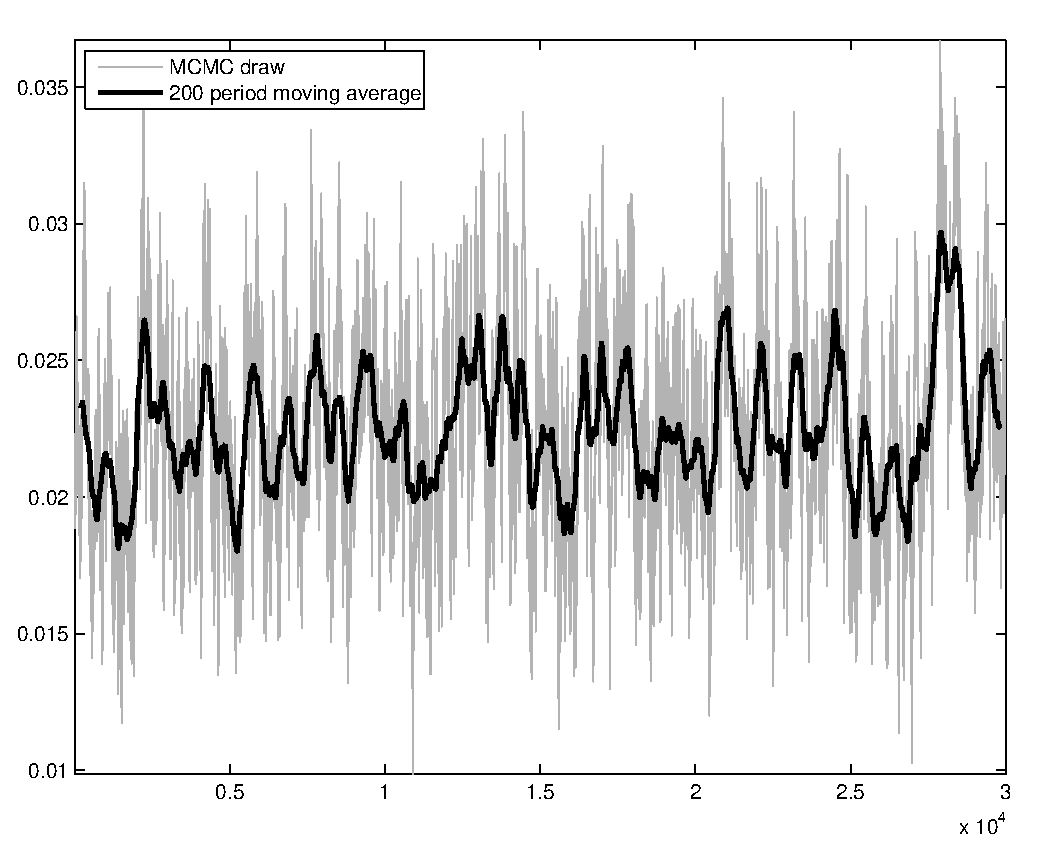
\includegraphics[scale=.35]{Bayesian_Estimation/RBC_high_acceptance/graphs/TracePlot_SE_eps_z}
  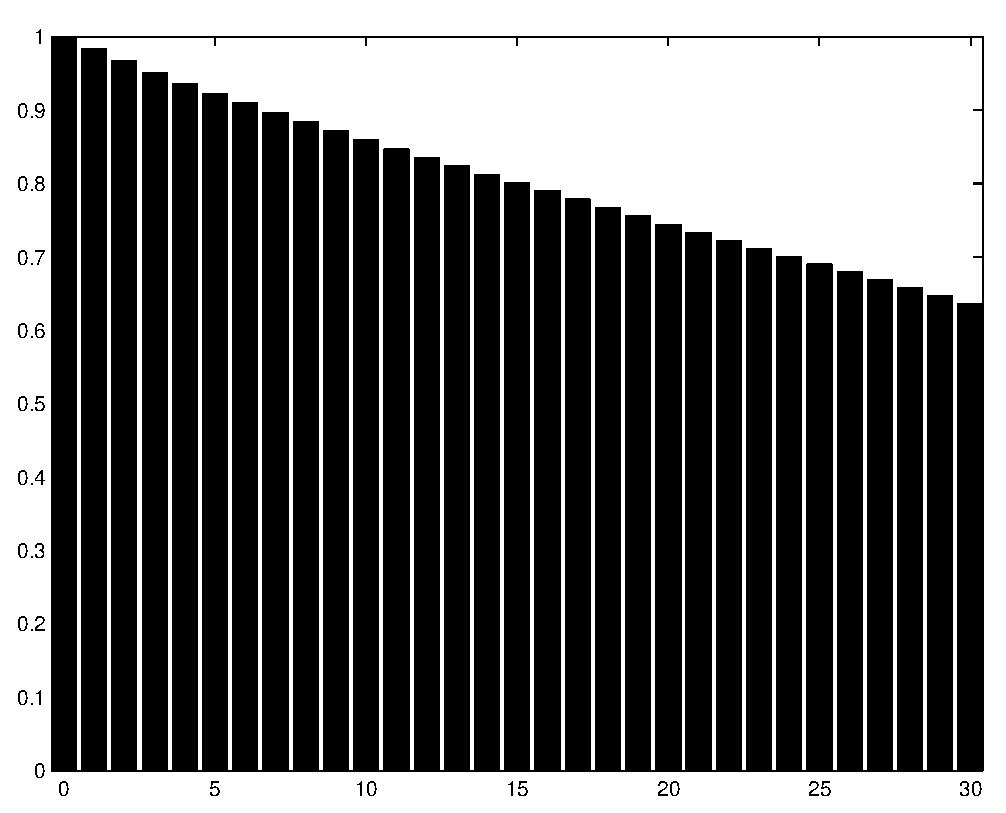
\includegraphics[scale=.35]{Bayesian_Estimation/RBC_high_acceptance/graphs/MH_Autocorrelation_SE_eps_z}
  \caption{Trace and Autocorrelation Plot: \texttt{eps\_z}}
\end{figure}
\begin{itemize}
    \item Acceptance Rate of 85\%
    \item Bad mixing and autocorrelation function only decays slowly
\end{itemize}
\end{frame}

\begin{frame}{Acceptance rate on target}
\begin{figure}
  
\includegraphics[scale=.30]{Bayesian_Estimation/RBC_medium_acceptance/graphs/TracePlot_SE_eps_z}
  
\includegraphics[scale=.30]{Bayesian_Estimation/RBC_medium_acceptance/graphs/MH_Autocorrelation_SE_eps_z}
  \caption{Trace and Autocorrelation Plot: \texttt{eps\_z}}
\end{figure}
\begin{itemize}
    \item Acceptance Rate of 21\%
    \item Good mixing and autocorrelation function decays relatively fast
\end{itemize}
\end{frame}

\section[Diagnostics]{Convergence and efficiency}



\begin{frame}[fragile]{Diagnostics: trace plots}
\begin{figure}
  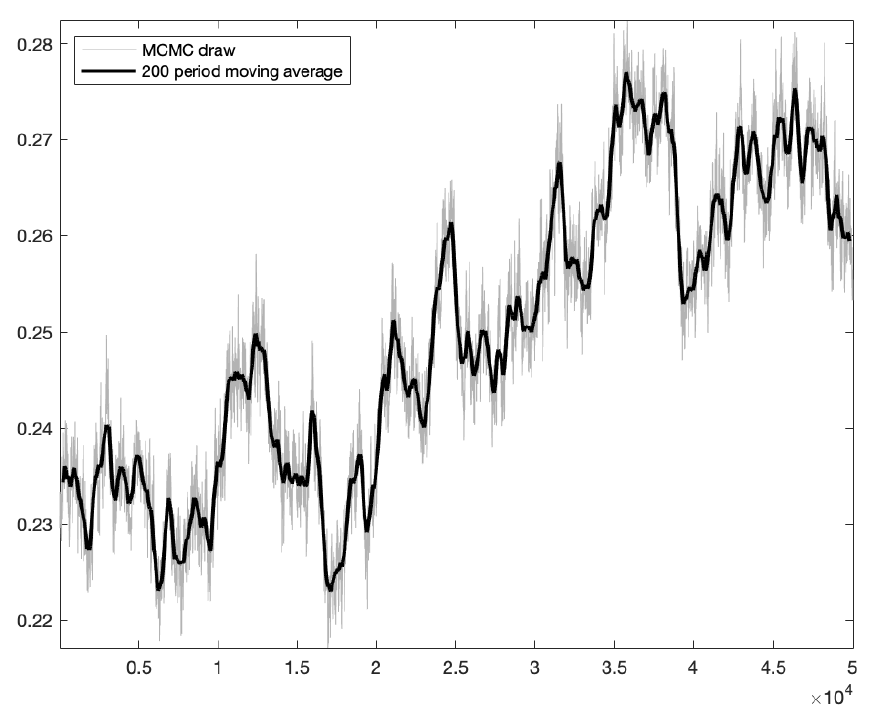
\includegraphics[width=5.2cm]{Figures/trace_plot}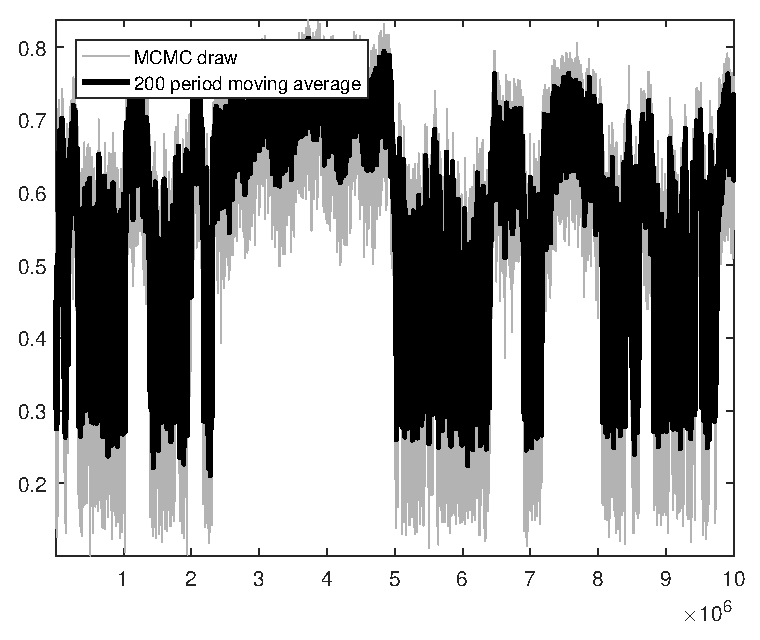
\includegraphics[width=5cm]{Figures/TracePlot_omega}
\end{figure}
\begin{witemize}
\item Trace plots available via
\begin{minted}{c++}
generate_trace_plots(chain_number)
\end{minted}
provide valuable clues to non-convergence\\
$\rightarrow$ e.g.\ drifts to regions of higher posterior density (left) or multi-modality (right)
\end{witemize}

\end{frame}

\begin{frame}{Efficiency}
\begin{witemize}
    \item Ideally, we want iid draws from the posterior
    \item MCMC only delivers correlated draws (hence: Markov Chain)
    \item While high autocorrelation in the draws may signify problems with the scaling, even with the ``optimal'' acceptance rate, there might be high autocorrelation
 \end{witemize}
\end{frame}


\begin{frame}{More powerful posterior samplers}
\begin{columns}<.->[T] % align columns
\begin{column}<.->{0.63\textwidth}
\begin{witemize}
    \item What if Markov Chain shows poor behavior: drift, high autocorrelation, poor mixing, large inefficiency factors?
    \item Try a more powerful \texttt{posterior\_sampling\_method}:
    \begin{enumerate}
      \item \texttt{\textquotesingle slice\textquotesingle}: Slice sampler
      \item \texttt{\textquotesingle tailored\_random\_block\_metropolis\_hastings\textquotesingle}: Tailored Random Block Metropolis Hastings (TaRB) of \textcite{Chib2010}
      \item \texttt{\textquotesingle dime\_mcmc\textquotesingle}: Differential-Independence Mixture Ensemble (DIME) sampler of \textcite{Boehl2022}
      \item \texttt{\textquotesingle hssmc\textquotesingle}: Sequential
Monte-Carlo sampler of \textcite{HerbstSchorfheide2014}
     \item \texttt{\textquotesingle dsmh\textquotesingle}: Dynamic Striated Metropolis Hastings sampler of \textcite{WaggonerEtAl2016}
    \end{enumerate}
\end{witemize}
\end{column}%
\hfill%
\begin{column}<1->{0.37\textwidth}
\begin{figure}
  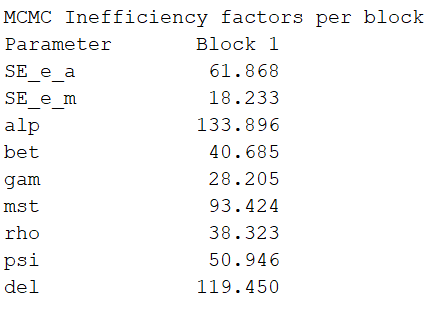
\includegraphics[scale=.55]{Figures/inefficiency_factors}
\end{figure}

\end{column}%
\end{columns}
\begin{itemize}
  \item Tend to be computationally more expensive but require less tweaking
\end{itemize}
\end{frame}

\begin{frame}{Tailored Random Block Metropolis Hastings (TaRB)}

\begin{witemize}
    \item Triggered using\\
    \texttt{posterior\_sampling\_method=\textquotesingle  tailored\_random\_block\_metropolis\_hastings\textquotesingle}
    \item Basic idea employ multiple-block MH algorithm by grouping parameters into distinct blocks and sequentially update each block by a MH step
    \item Correlated parameters should be put into same block, uncorrelated sets in different blocks
    \item Problem: correlation structure a priori unknown
    \item Solution: randomly assign parameters to blocks, with the \texttt{posterior\_sampler\_options} name/value pair \texttt{(new\_block\_probability,double)} governing probability of new block
    \item For each MH step: run additional mode-finding step and compute (approximation) to Hessian\\
    $\rightarrow$ powerful for finding true mode, but computationally expensive
\end{witemize}

\end{frame}

\begin{frame}{Monitoring convergence}
\begin{witemize}
    \item We only want to consider draws after the transition kernel has converged to the invariant distribution
    \item How to monitor that?
    \begin{enumerate}
      \item \textcite{Geweke1992} convergence diagnostics: requires single MCMC
      \item \textcite{BrooksGelman1998} convergence diagnostics: requires at least two MCMC
      \item \textcite{RafteryLewis1992} convergence diagnostics: can be requested using the \\ \texttt{raftery\_lewis\_diagnostics}-option
    \end{enumerate}
\end{witemize}
\end{frame}

\subsection{1.\ \textcite{Geweke1992} Convergence Diagnostics}
\renewcommand{\Source}{\textcite{Geweke1992}}
\begin{frame}{1.\ \textcite{Geweke1992} Convergence Diagnostics}
\begin{itemize}
    \item Idea: if we have sufficient number of draws from posterior, the first $S_A$ draws after a burn-in of $S_0$ should be similar to the last $S_C$ draws
    \item By leaving out $S_B$ draws in the middle, draws in $S_A$ and $S_C$ should be independent
    \item In practice, often $S_A=0.1S_1$, $S_C=0.4S_1$, where $S_1$ is the number of draws after the burn-in
    \item To test similarity, test the means (or any other statistics) $g_{S_i}=E(g(\theta)|Y^T),i \in \{A,C\} $:
    \begin{equation}
          C{D_{GWK}} = \frac{{{{\hat g}_{{S_A}}} - {{\hat g}_{{S_C}}}}}{{\frac{{{{\hat \sigma }_A}}}{{\sqrt {{S_A}} }} + \frac{{{{\hat \sigma }_C}}}{{\sqrt {{S_C}} }}}}
    \end{equation}
    \item This is a two-sample t-test and thus asymptotically
    \begin{equation}
    CD_{GWK} \to N\left( {0,1} \right)
    \end{equation}
    \item Problem: estimate of numerical standard error $\hat \sigma_i$ needs to take correlation in draws into account
    \item Use \textcite{NeweyWest1987}-type estimator that tapers spectral density
\end{itemize}
\end{frame}
\note{Alternatively, as Dynare does it, the square is Ch2 distributed}


\renewcommand{\Source}{}
\begin{frame}{Example}
\begin{figure}
  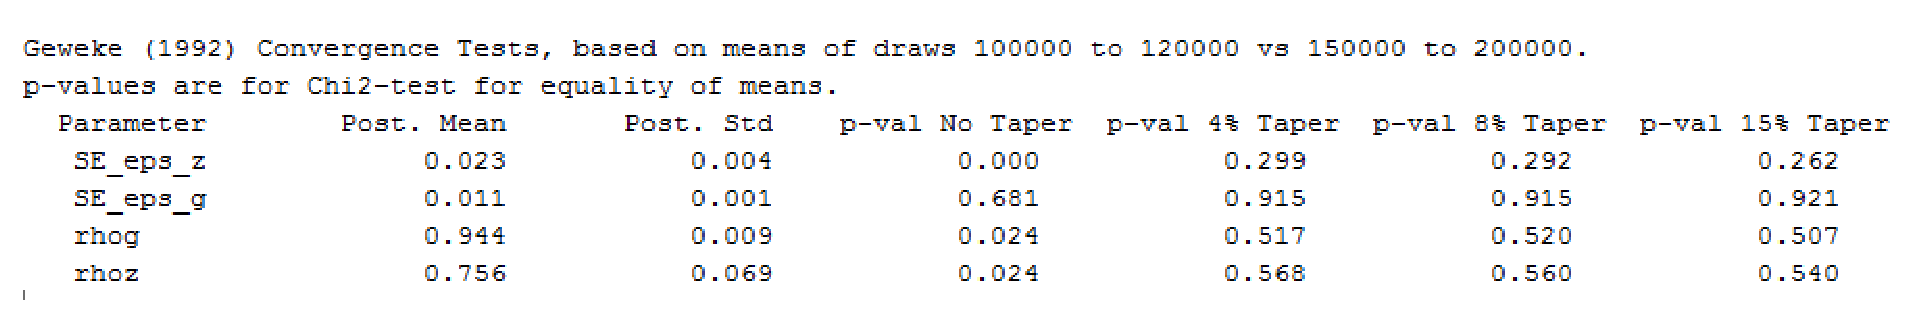
\includegraphics[scale=.45]{Figures/geweke_diagnostics}
\end{figure}
\begin{itemize}
    \item Higher tapers correcting for serial correlation suggest convergence
\end{itemize}
\end{frame}

\subsection{2.\ \textcite{BrooksGelman1998} Convergence Diagnostics}
\renewcommand{\Source}{\textcite{BrooksGelman1998}}
\begin{frame}{2.\ \textcite{BrooksGelman1998} Convergence Diagnostics}
\begin{witemize}
    \item Idea: wherever the MC starts, it should converge to the same invariant distribution
    \item Start multiple chains from \highlight{over-dispersed draws} and see whether they yield similar posterior draws after burn-in
    \item The univariate convergence diagnostics are based on comparing \highlight{pooled} and \highlight{within} MCMC moments (ANOVA)
    \item Consider a statistic $g$ with variance $\sigma$ and having $J$ chains with $N$ draws each after discarding a burn-in
    \item Denote means with bars
    \item The \highlight{variance within a chain} is given by
    \begin{equation}
    {\sigma _j^2} = \frac{1}{{N - 1}}\sum\limits_{n = 1}^N {{{\left( {{g_{nj}} - {{\bar g}_j}} \right)}^2}}
    \end{equation}
\end{witemize}
\end{frame}

\begin{frame}{Getting the variances}
\begin{itemize}
    \item The \highlight{between sequence variance} $B/N$ is given by
    \begin{equation}
    \frac{B}{N} = \frac{1}{{J - 1}}\sum\limits_{j = 1}^J {{{\left( {{{\bar g}_j} - \bar g} \right)}^2}}
    \end{equation}
    \item Here, $B/N$ is the square of the standard error of the mean and $B$ the actual variance estimate of $g$
    \item The (average) \highlight{within sequence variance} is given by
    \begin{equation}
    W = \frac{1}{{J\left( {N - 1} \right)}}\sum\limits_{j = 1}^J {\sum\limits_{n = 1}^N {{{\left( {{{\bar g}_{jn}} - {{\bar g}_j}} \right)}^2}} }  = \frac{1}{J}\sum\limits_{j = 1}^J \sigma _j^2
    \end{equation}
\item The variance $\sigma^2$ can now be estimated by a weighted average of the two:
\begin{equation}
{{\hat \sigma }^2} = \left( {1 - \frac{1}{N}} \right)W + \frac{{1 + J}}{{NJ}}B
\end{equation}
\item Because we use over-dispersed starting points, this is an overestimate of $\sigma^2$, but it is consistent
\end{itemize}
\end{frame}

\begin{frame}{Potential scale reduction factor}
\begin{itemize}
    \item The statistic of interest is the \highlight{potential scale reduction factor}, i.e.\ the ratio between the pooled variance estimate and the within-chain variance estimate:
    \begin{equation}
    \hat R = \sqrt \frac{{{{\hat \sigma }^2}}}{W}
    \end{equation}
    \item If $\hat R$ is large, either the pooled variance estimate $\hat \sigma^2$ can be decreased by further simulations or the within chain variance will increase due to it not yet having made a full tour through the target distribution
    \item If $\hat R$ is close to 1, each of the $J$ chains of $N$ draws is close to the target distribution
    \item At convergence, three properties should hold
    \begin{itemize}
      \item $\hat R$ should be close to 1
      \item The pooled variance $\hat \sigma^2$ should stabilize with convergence as the chains were started from an over-dispersed distribution
      \item The same should hold true for the within chain variance, which should be smaller than $\hat \sigma^2$
    \end{itemize}
    \item All three conditions can be monitored graphically
\end{itemize}
\end{frame}

\begin{frame}{A non-parametric version}
\begin{witemize}
    \item But: previous approach assumes normality by looking at means and variances
    \item Alternative (also used in Dynare): take length of the $1-\alpha$ percentile for each of the chains and for the pooled draws
    \item Compare the interval for the pooled draws with the average from the individual chains
    \begin{equation}
    \hat R_{interval} = \frac{\text{length of total sequence interval}}{\text{mean length of within sequence interval}}
    \end{equation}
    \item $R_{interval}$ is a \highlight{potential scale reduction factor} based on percentiles
    \item The same convergence criteria apply
\end{witemize}
\end{frame}


\begin{frame}{Example}
\begin{figure}
  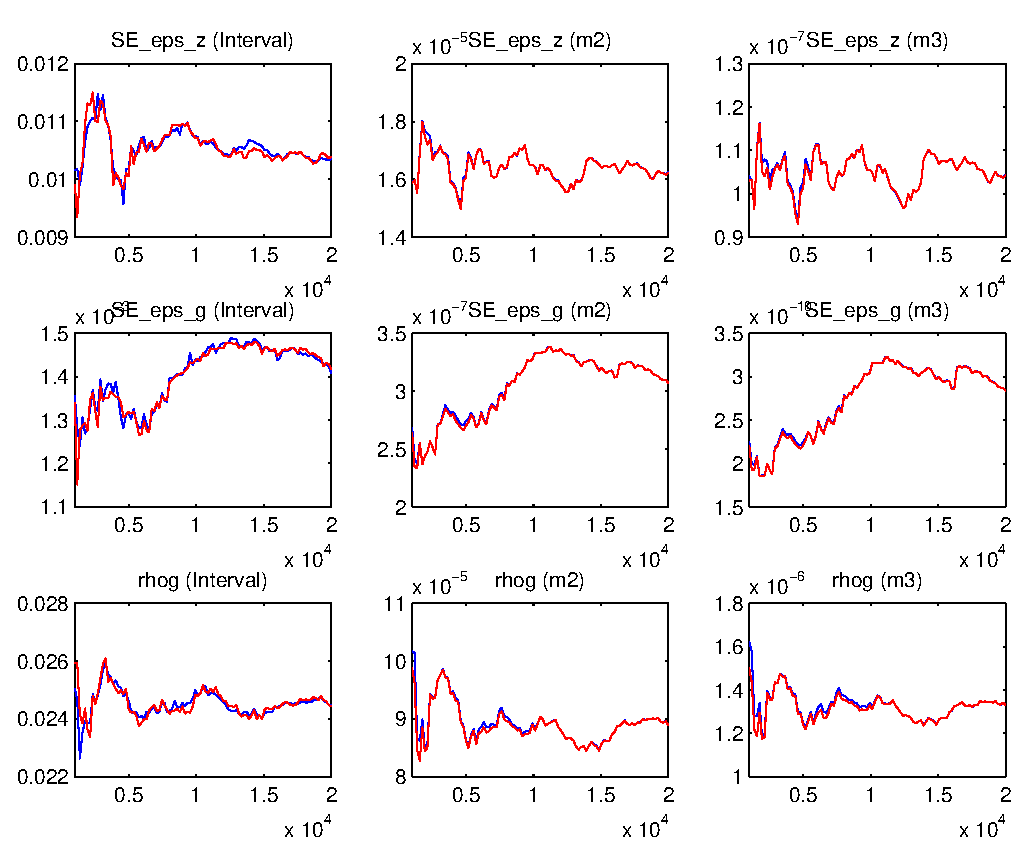
\includegraphics[scale=.55]{Figures/RBC_Bayesian_udiag1_300000.eps}
\end{figure}
\end{frame}

\subsection{3.\ \textcite{RafteryLewis1992} Convergence Diagnostics}

\renewcommand{\Source}{\textcite{RafteryLewis1992}}
\begin{frame}{3.\ \textcite{RafteryLewis1992} convergence diagnostics}
\begin{witemize}
    \item The question: how many draws do we need to make sufficiently precise statements about a quantile of a posterior function $U(\theta)$?
    \item Applicable to any function $U()$, but we take $U(\theta)=\theta$
    \item Want to estimate quantile $q$ to within $\pm r$ with probability $s$
    \item Typically: $q=0.025$, $r=0.0125$, $s=0.95$\\
    $\rightarrow$ want reported 95\% HPDIs of $U$ to have actual posterior probability between 92.5\% and 97.5\%
    \item To do so, we drop $M$ draws as a burn-in and then take $N$ draws of which we use every $k^{th}$ one
    \item Central idea: construct Markov Chain out of $U(\theta_t)$ and then use Markov-Chain theory
    \item Helpful derivations are provided in \textcite[][SI 6]{TrairatphisanEtAl2014} and \href{http://www.statslab.cam.ac.uk/~rrw1/markov/M.pdf}{Richard Weber's course notes}
\end{witemize}
\end{frame}


\begin{frame}{Discretization and finding thinning factor $k$}
\begin{witemize}
    \item First step: create binary indicator of whether a draw is below or above the cutoff value $u$ of the $q^{th}$ percentile
    \begin{equation}
    Z_t = \left\{ {\begin{array}{*{20}{c}}
  {1, \text{ if } U(\theta_t)\leqslant u} \\
  {0 \text{ otherwise}}
\end{array}} \right.
\end{equation}
    \item $Z_t$ is typically not a Markov Chain, but thinned process $\left\{Z_t^{(k)}\right\}$, where we only take every $k^{th}$ draw, will typically approximate Markov Chain for sufficiently large $k$
    \item Find $k$ by likelihood ratio test between second- and first-order Markov model\\
    $\rightarrow$ take smallest $k$ for which first-order model fits better
    \item Next step: find burn-in $M$
\end{witemize}
\end{frame}

\begin{frame}{Finding the burn-in $M$ I}
\begin{itemize}
    \item Denote the transition matrix for $\left\{Z_t^{(k)}\right\}$ with
    \begin{equation}
    P = \left( {\begin{array}{*{20}{c}}
  {1 - \alpha }&\alpha  \\
  \beta &{1 - \beta }
\end{array}} \right)
\end{equation}
\item The stationary distribution is given by
\begin{equation}
\pi  = \left( {\begin{array}{*{20}{c}}
  {{\pi _0}} \\
  {{\pi _1}}
\end{array}} \right) = \frac{1}{{\alpha  + \beta }}\left( {\begin{array}{*{20}{c}}
  \alpha  \\
  \beta
\end{array}} \right)
\end{equation}
and the $l$-step transition matrix by
\begin{equation}
{P^l} = \left( {\begin{array}{*{20}{c}}
  {{\pi _0}}&{{\pi _1}} \\
  {{\pi _0}}&{{\pi _1}}
\end{array}} \right) + \frac{{{\lambda ^l}}}{{\alpha  + \beta }}\left( {\begin{array}{*{20}{c}}
  \alpha &{ - \alpha } \\
  { - \beta }&\beta \: ,
\end{array}} \right)
\end{equation}
where $\lambda=1-\alpha-\beta$
\end{itemize}
\end{frame}

\begin{frame}{Finding the burn-in $M$ II}
\begin{itemize}
    \item We want a burn-in so that after $m$ draws, we are within $\varepsilon$ of stationary distribution, i.e.
    \begin{equation}
    P\left(Z_m^{(k)}=i|Z_m^{(0)}=j\right)=e_jP^me_i^T
    \end{equation}
    to be within $\varepsilon$ of $\pi_i$ for all $i,j$ (where $e_i$ denotes Euclidean basis vector)
    \item This is satisfied for
    \begin{equation}
    {\lambda ^m} \leqslant \frac{{\left( {\alpha  + \beta } \right)\varepsilon }}{{\max \left( {\alpha ,\beta } \right)}} \Leftrightarrow m = \frac{{\log \left( {\frac{{\left( {\alpha  + \beta } \right)\varepsilon }}{{\max \left( {\alpha ,\beta } \right)}}} \right)}}{{\log \lambda }}
    \end{equation}
    \item Thus
    \begin{equation}
      M=mk
    \end{equation}
    \item Dynare uses $\varepsilon=0.001$
\end{itemize}
\end{frame}

\begin{frame}{Finding the required number of draws $N$}
\begin{itemize}
    \item The quantile estimate is given by
    \begin{equation}
    {\bar{Z}}_t^{\left( k \right)}\equiv \hat P\left( {U \leqslant u} \right) = \frac{1}{n}\sum\limits_{t = 1}^n {Z_t^{\left( k \right)}}
    \end{equation}
    \item For large $n$, it is approximately normally distributed with mean $q$ and variance
    \begin{equation}
    \frac{1}{n}\frac{{\left( {2 - \alpha  - \beta } \right)\alpha \beta }}{{{{\left( {\alpha  + \beta } \right)}^3}}}
    \end{equation}
    \item Requirement $P\left(q-r \leq {\bar{Z}}_t^{\left( k \right)} < q+r \right)=s$ implies
    \begin{equation}
    n = \frac{{\left( {2 - \alpha  - \beta } \right)\alpha \beta }}{{{{\left( {\alpha  + \beta } \right)}^3}}}\left( {\frac{{{\Phi ^{ - 1}}\left( {\frac{1}{2}\left( {s + 1} \right)} \right)}}{r}} \right) \: ,
    \end{equation}
    where $\Phi^{ - 1}$ is the inverse standard normal CDF
    \item Thus
    \begin{equation}
    N=nk
    \end{equation}
\end{itemize}
\end{frame}


\renewcommand{\Source}{}
\begin{frame}{Example}
\begin{figure}
  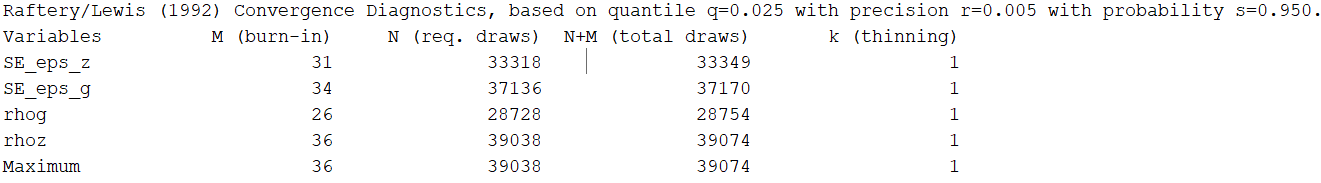
\includegraphics[scale=1.3]{Figures/Raftery_Lewis}
\end{figure}
\begin{itemize}
    \item Can be requested using the \texttt{raftery\_lewis\_diagnostics}-option
\end{itemize}
\end{frame}


\begin{frame}{Prior vs. posterior plots}{\texttt{\texttt{RBC\_Bayesian.mod}}}
\begin{figure}
  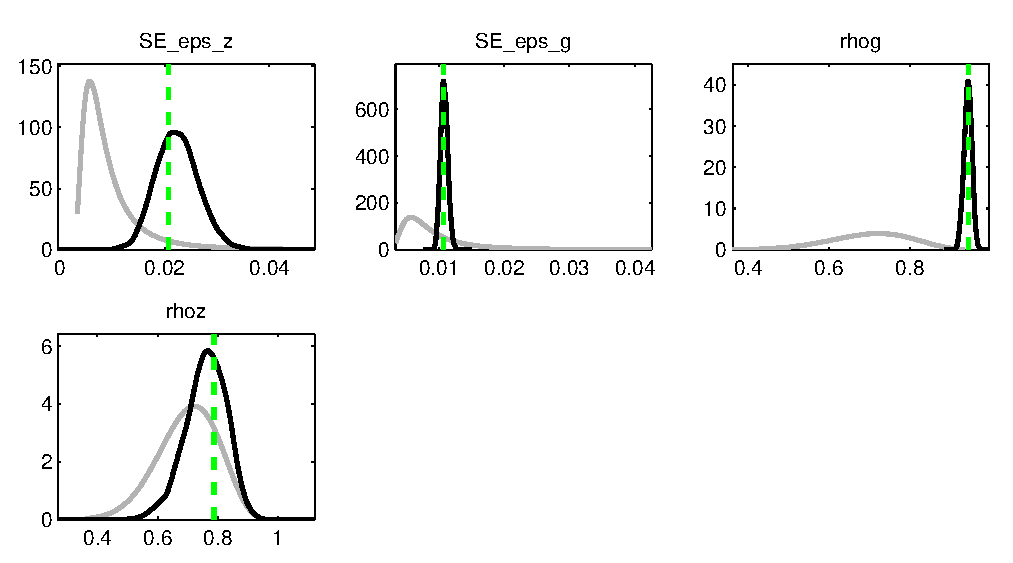
\includegraphics[scale=.55]{Bayesian_Estimation/RBC_medium_acceptance/Output/RBC_medium_acceptance_PriorsAndPosteriors1}\\
\end{figure}
\begin{itemize}
    \item Priors (grey) and posteriors (black) differ: data seems to be informative for updating
    \item Exception: $\rho_z$ where we saw the flat likelihood
    \item When the prior is (almost) equal to the posterior, there are two cases
    \begin{itemize}
      \item Data is uninformative
      \item Data is informative, but coincides with chosen prior
    \end{itemize}
\end{itemize}
\end{frame}



\part{References}
%%
\begin{frame}[allowframebreaks]{Bibliography}
\printbibliography
\end{frame}
\end{document}
